%%%%%%%%%%%%%%%%%%%%%%%%
%% Sample use of the infthesis class to prepare a thesis. This can be used as 
%% a template to produce your own thesis.
%%
%% The title, abstract and so on are taken from Martin Reddy's csthesis class
%% documentation.
%%
%% MEF, October 2002
%%%%%%%%%%%%%%%%%%%%%%%%

%%%%
%% Load the class. Put any options that you want here (see the documentation
%% for the list of options). The following are samples for each type of
%% thesis:
%%
%% Note: you can also specify any of the following options:
%%  logo: put a University of Edinburgh logo onto the title page
%%  frontabs: put the abstract onto the title page
%%  deptreport: produce a title page that fits into a Computer Science
%%      departmental cover [not sure if this actually works]
%%  singlespacing, fullspacing, doublespacing: choose line spacing
%%  oneside, twoside: specify a one-sided or two-sided thesis
%%  10pt, 11pt, 12pt: choose a font size
%%  centrechapter, leftchapter, rightchapter: alignment of chapter headings
%%  sansheadings, normalheadings: headings and captions in sans-serif
%%      (default) or in the same font as the rest of the thesis
%%  [no]listsintoc: put list of figures/tables in table of contents (default:
%%      not)
%%  romanprepages, plainprepages: number the preliminary pages with Roman
%%      numerals (default) or consecutively with the rest of the thesis
%%  parskip: don't indent paragraphs, put a blank line between instead
%%  abbrevs: define a list of useful abbreviations (see documentation)
%%  draft: produce a single-spaced, double-sided thesis with narrow margins
%%
%% For a PhD thesis -- you must also specify a research institute:
\documentclass[mscres, lfcs, logo]{infthesis}

%% For an MPhil thesis -- also needs an institute
% \documentclass[mphil,ianc]{infthesis}

%% MSc by Research, which also needs an institute
% \documentclass[mscres,irr]{infthesis}

%% Taught MSc -- specify a particular degree instead. If none is specified,
%% "MSc in Informatics" is used.
% \documentclass[msc,cogsci]{infthesis}
% \documentclass[msc]{infthesis}  % for the MSc in Informatics

%% Master of Informatics (5 year degree)
% \documentclass[minf]{infthesis}

%% Undergraduate project -- specify the degree course and project type
%% separately
% \documentclass[bsc]{infthesis}
% \course{Artificial Intelligence and Psychology}
% \project{Fourth Year Project Report}

%% Put any \usepackage commands you want to use right here; the following is 
%% an example:
\usepackage{natbib}
\usepackage{amsfonts}
\usepackage{amssymb}
\usepackage{listings}
\usepackage{color}
\usepackage{verbatim}

\newcounter{nalg}[chapter] % defines algorithm counter for chapter-level
\renewcommand{\thenalg}{\thechapter .\arabic{nalg}} %defines appearance of the algorithm counter
\DeclareCaptionLabelFormat{algocaption}{Algorithm \thenalg} % defines a new caption label as Algorithm x.y

\lstnewenvironment{algorithm}[1][] %defines the algorithm listing environment
{   
    \refstepcounter{nalg} %increments algorithm number
    \captionsetup{labelformat=algocaption,labelsep=colon} %defines the caption setup for: it ises label format as the declared caption label above and makes label and caption text to be separated by a ':'
    \lstset{ %this is the stype
        mathescape=true,
        frame=tB,
        numbers=left, 
        numberstyle=\scriptsize,
        basicstyle=\footnotesize, 
        keywordstyle=\color{black}\bfseries\em,
        keywords={,input, output, and, or, if, then, else, foreach, in, do, begin, end, } %add the keywords you want, or load a language as Rubens explains in his comment above.
        morecomment=[l]{//}, % l is for line comment
        commentstyle=\itshape\color{green},
        numbers=left,
        xleftmargin=.04\textwidth,
        #1 % this is to add specific settings to an usage of this environment (for instnce, the caption and referable label)
    }
}
{}

%% Some custom commands:
\newcommand{\ket}[1]{\vert #1 \rangle}

%% Information about the title, etc.
\title{Towards Distributed Quantum Algorithms}
\author{Pablo Andres-Martinez}

%% If the year of submission is not the current year, uncomment this line and 
%% specify it here:
% \submityear{1785}

%% Optionally, specify the graduation month and year:
% \graduationdate{February 1786}

%% Specify the abstract here.
\abstract{%
}

%% Now we start with the actual document.
\begin{document}

%% First, the preliminary pages
\begin{preliminary}

%% This creates the title page
\maketitle

%% Acknowledgements
\begin{acknowledgements}
\end{acknowledgements}

%% Next we need to have the declaration.
\standarddeclaration

%% Finally, a dedication (this is optional -- uncomment the following line if
%% you want one).
% \dedication{To my mummy.}

%% Create the table of contents
\tableofcontents

%% If you want a list of figures or tables, uncomment the appropriate line(s)
% \listoffigures
% \listoftables

\end{preliminary}

\chapter{Introduction}
\label{chap:Introduction}

In this thesis, we propose an algorithm for the automated translation of programs from monolithic quantum computers to distributed grids of quantum computers. The reader is not required to have any prior knowledge of quantum computing, as we will introduce the concepts needed in this thesis in an incremental manner. In some occasions, we will use analogies from classical computer science -- ranging from distributed architectures to compilers -- that should help understand the key concepts of distributed quantum computing. Our main contribution consists in reducing the problem of efficiently distributing a quantum circuit to the problem of hypergraph partitioning, which is a problem thoroughly studied in the literature of classical computer science.

Quantum computing aims to take advantage of quantum mechanics to speed-up computations. There are many examples of problems that, although solvable by a classical computer, the time it would take to compute them is unreasonable in practice, regardless how large or fast your classical computer is. Some of these \textit{intractable problems} can be solved efficiently on a quantum computer. Well-known examples of such problems are:

\begin{itemize} 
\item \textit{Factorisation of large numbers}: In classical computers, all known factorisation algorithms take exponential time with respect to the input size. It is strongly believed that there is no way a classical computer can solve the problem efficiently -- in fact, we are so confident about it that most widely used encryption systems, like RSA, rely on this. However, quantum computers are capable of solving that problem in polynomial time (i.e.\ making it tractable), using Shor's algorithm~\citep{Shor}.
\item \textit{Unstructured search}: The aim is to perform a brute-force search (i.e.\ requiring no prior knowledge about the search space) over \(N\) data-points. Classical computers have no other option than testing each data-point, so the time they take to perform the search is proportional to \(N\). With a quantum computer, using Grover's algorithm~\citep{Grover}, the search is done in time proportional to \(\sqrt{N}\).
\end{itemize}

Besides, a recent result by \citet{BQPSepPH} gives formal proof of the existence of a large family of problems that a classical computer may never solve in polynomial time, but are solvable in polynomial time on a quantum computer. Nevertheless, all of these results are theoretical in nature, and giving experimental evidence of this gap in computational power is a highly active area of research, known as \textit{quantum supremacy}. 

Quantum computing would be very valuable in many areas of research that deal with problems that are intractable on classical computers. Some of the main applications that have been discussed in the literature are:

\begin{itemize}
\item \textit{Chemistry, medicine and material sciences}: Calculating molecular properties on complex systems is extremely demanding for classical computers. However, polynomial algorithms for this kind of problems are known for quantum computers~\citep{TowardsQuantumChemistry}. %Quantum computers are likely to trigger a revolution on areas of science that need to model molecules and their interactions.
\item \textit{Machine learning}: Finding patterns in a large pool of data is the essence of machine learning. Multiple quantum algorithms have been shown to be able to detect patterns that are believed not to be efficiently attainable classically~\citep{QuantumMachineLearning}.
\item \textit{Engineering}: Optimisation and search problems are common in almost every area of engineering. Quantum computers are particularly well suited for these tasks, with Grover's algorithm (unstructured search) being an obvious example.
\end{itemize}

For any of these applications we will require large scale quantum computers. Due to the obstacles in the way of building a large quantum computer, some experts have advocated the alternative of building a \textit{quantum multicomputer}: a grid of small quantum computers that cooperate to perform an overall computation~\citep{DistributedQCHW}. Small quantum computers have already been built, and the technology needed to connect them in a grid is known. Thus, it is possible that large scale grids of quantum computers become available before large monolithic quantum computers do. Even if this were not the case, distributed quantum computing would still be a desirable asset, for similar reasons it is for classical computing: a cluster of small computers may be cheaper than a large mainframe, and a multicomputer is intrinsically modular, so we may easily adjust the amount of resources we dedicate to a computation.

Unfortunately, there is virtually no support for developing programs to be run on distributed quantum architectures. The literature on quantum algorithms and quantum programming languages focuses almost exclusively on a single model of quantum computation -- the circuit model --, meant to be run on a monolithic computer. In this thesis, we intend to make a first step towards the spread of distributed quantum algorithms, providing an automated method for distributing any input circuit across an arbitrary number of quantum computers.

\section{Outline of the chapters}

Chapters~\ref{chap:Overview} and~\ref{chap:Distributed} correspond to the literature review relevant to this thesis, and they identify the problem we intend to solve. Chapter~\ref{chap:Overview} introduces the key concepts of quantum computer science that will be required throughout this thesis. Most importantly, \S\ref{Principles} explains the principles of quantum computing, and gives an intuition behind the speed-up it achieves; while \S\ref{Hardware} discusses the scalability challenges of quantum computers, and presents the main model of quantum computing -- the circuit model. Chapter~\ref{chap:Distributed} gives an introduction to distributed quantum computing: In \S\ref{Ebits} we explain how quantum information may be communicated across QPUs, \S\ref{IntroDistributing} reviews the main paper our thesis is built upon~\citep{NonLocalCNOT}, and \S\ref{DQC_Architecture} describes an abstract distributed quantum architecture.

Our contributions are presented in Chapter~\ref{chap:Project}. First, in \S\ref{NonLocalGates} we propose two extensions of the work by \citet{NonLocalCNOT}. \S\ref{EfficientDistrib} is the core of the thesis, where we describe our algorithm for automated distribution of quantum circuits. We present our first version of the algorithm, then we describe its two extensions, corresponding to the ones we proposed in \S\ref{NonLocalGates}. \S\ref{Interchange} outlines a third potential extension that we propose as further work.

Finally, in Chapter~\ref{chap:Results}, we present the results of using our algorithm to distribute different benchmark circuits drawn from the literature. We discuss these results and study the effect of both extensions of our algorithm. Chapter~\ref{chap:Conclusions} ends the thesis by drawing some conclusions and suggesting further work.
\chapter{Quantum Computing: A brief overview}
\label{chap:Overview}

\section{The principles of quantum computing}
\label{Principles}

The advantages of using quantum mechanics to perform computations come down to the following three principles:

\begin{itemize}

\item \textit{Superposition}: In classical computing, the unit of information is the \textit{bit}, which may take one of two values: \(0\) or \(1\). In quantum computing, the \textit{bit}'s counterpart is the \textit{qubit}, whose value may be \textit{any linear combination} of the \(0\) state and the \(1\) state, known as a \textit{superposition}, and usually written as: \[\ket{qubit} = \alpha\ket{0} + \beta\ket{1}\] where \(\alpha\) and \(\beta\) are complex numbers that must satisfy: \(\alpha^2 + \beta^2 = 1\).

A popular analogy of a qubit's superposition is a coin spinning\footnote{Note this is just an analogy, and while a coin spinning can be perfectly described using classical physics, a qubit can not.}: the classical states (\(0\) and \(1\)) are \textit{heads} and \textit{tails}, but when the coin is spinning, its state is neither of them. If we knew exactly how the coin was spinning, we would be able to describe the probability of seeing heads or tails when it stops; these would be our \(\alpha^2\) and \(\beta^2\) values. Besides, we may \textit{measure} a qubit, and doing so corresponds in our analogy to abruptly stopping the coin, then checking if it is \textit{heads} or \textit{tails}. Through certain operations -- that would correspond to altering the axis of spin of the coin --, we may change the coefficients \(\alpha\) and \(\beta\) of the superposition. 

In most quantum programs, we encode input and read output (after measurement) as standard classical binary strings. Therefore, for input/output we use as many qubits as bits would be required. Superposition allows us to maintain -- during mid-computation -- a superposition of all potential solutions to the problem, and update all of them simultaneously with a single operation to the qubits. In some sense, superposition allows us to explore multiple choices/paths of the computation, using only the resources required to explore a single one of those paths. And the number of paths we can explore simulatenously can be up to exponential, as a collection of \(N\) qubits may be in a state of superposition of all the possible \(2^N\) classical states.

\item \textit{Interference}: As we just discussed, superposition gives us the ability to simultaneously explore different paths to solve a problem. However, in the end we will need to measure the qubits -- stop the coins -- and the result will be intrinsically random. For quantum computing to be any better than a probabilistic classical computer, we require the ability to prune the paths that have led to a result we do not want. This is precisely what \textit{interference} provides: some operations on the qubits may make different classical states in the superposition cancel each other out. Interference is at the core of any speed-up achieved by a quantum algorithm, and taking advantage of it is the main challenge when designing quantum algorithms.

\item \textit{Entanglement}: Quantum mechanics allows the possibility of having a pair of qubits \(a\) and \(b\) in a superposition such as: \[\ket{a,b} = \frac{1}{\sqrt{2}}\ket{0,0} + \frac{1}{\sqrt{2}}\ket{1,1}\] This implies that, when we measure the qubits, we may either read \(a=0, b=0\) or \(a=1, b=1\) as outcome, never \(a\not=b\) (the coefficients for \(\ket{0,1}\) and \(\ket{1,0}\) are both \(0\)). Then, what happens if we only measure \(a\)? In this particular case, we would also know \(b\)'s outcome, without measuring it. In short, acting on one qubit has an instantaneous effect on the other. Whenever a group of qubits exhibits this property, we say they are \textit{entangled}. Entanglement holds regardless how far apart \(a\) is from \(b\); for instance, they could be on two different quantum processing units of a distributed grid. Indeed, entanglement will be key in our discussion of distributed quantum algorithms, and we explain how to use it to perform non-local operations in \S\ref{IntroDistributing}.

\end{itemize}


\section{Building quantum computers}
\label{Hardware}

Physicists have come up with different ways of realising qubits in labs. The key idea is to find a physical system that displays non-classical behaviour, and put it under the appropriate circumstances so we can manage its quantum properties. At the same time, we must ensure that noise from the environment does not interfere with our quantum information. \citet{ArchitectureSurvey} give an excellent survey of the state of the art of quantum architectures. Among these, the three most developed are:

\begin{itemize}

\item \textit{Quantum optics}: The state of a qubit is represented in the properties of photons, for instance, their polarization~\citep{OpticsQC}. A great advantage of this technology is that photons can be easily sent over long distances, while preserving their quantum state. Thus, protocols in quantum information that heavily rely on communication, such as Quantum Key Distribution~\citep{QKD}, are usually discussed and experimented with using quantum optics. The downside of this technology is that it is very difficult to make photons interact, which is required for universal computation.

\item \textit{Ion-traps}: Each qubit is embodied as an ion, confined inside a chamber by means of an electric or magnetic fields. The qubit is acted upon by hitting the ion with electromagnetic pulses (e.g.\ laser light or microwave radiation). Groups of experimentalists have proposed how to scale up the technology~\citep{HensingerIonTraps}, and are currently building prototypes.

\item \textit{Superconductors}: Small circuits, similar to classical electrical circuits, are cooled down to near absolute zero so the quantum interactions of electrons are not obscured by other perturbations. Different parts of the circuit encode different qubits, which can be acted upon by applying electric potentials. One of the main advantages of this approach is that the technology required for building the chips is fairly similar to the one for classical computer chips. This technology is the most experimentally developed. In fact, using it, both IBM and Intel have already built small generic-purpose quantum computers with 17-20 qubits.

\end{itemize}

However, for quantum computers to be useful in real world applications, their qubit count should increase, at the very least, one order of magnitude. And, unfortunately, increasing the amount of qubits in a quantum computer is particularly difficult, due to some challenges we will now discuss.


\subsection{Scalability challenges}
\label{Challenges}

There are two main challenges to overcome in order to build large scale quantum computers:

\begin{itemize}

\item \textit{Decoherence}: In \S\ref{Principles} we discussed the importance of having superposition in quantum computing, and we compared a qubit in superposition with a coin spinning. For similar reasons why a coin spinning will eventually stop, a qubit in superposition will eventually degenerate into a classical state (i.e.\ either \(\ket{0}\) or \(\ket{1}\)). This phenomenon is known as \textit{decoherence}. Experimentalists attempt to increase the time it takes for the state of the qubit to degenerate\footnote{A fundamentally different approach, \textit{anyonic} (a.k.a.\ topological) quantum computing, has been proposed to avoid the problem of decoherence altogether. It would use physical systems that, theoretically, can be completely protected against decoherence~\citep{Anyonic}. Although promising, currently this proposal has little experimental underpinning, and it is not regarded as attainable in the near future.}. Decoherence is the main constraint to scalability for quantum computers, as it limits the lifespan of qubits, limiting the number of operations that can be applied in a single program. 

Certainly, the state of bits also degenerates in classical computers. However, in their case this is easier to account for: we can monitor the bits, and make sure to correct any unwanted change. This is not so simple in quantum computers, as monitoring a qubit would require \textit{measuring} it, which destroys any quantum superposition. Nevertheless, it is still to some extent possible to protect our quantum state from errors -- either due to decoherence or imperfect hardware -- through specialised quantum error correction routines~\citep{QuantumErrorCorrection}. This is a very active area of research, and it will be essential for the implementation of reliable large scale quantum computers.


\item \textit{Connectivity}: In order to run any computation on qubits, we will need to be able to apply multi-qubit operations on any subset of the computer's qubits. However, it is not realistic to expect that quantum computers will have fast connectivity between all qubits, for instance due to spatial separation of these in the hardware. In classical systems, the same problem is solved by a memory hierarchy, with a ceaseless flow of data going up and down of it, from main memory to registers (where computation is performed) and back. The memory hierarchy model works because data can stay idly in main memory while computation on the registers is carried out. However, in quantum computers we must avoid qubits being idle, as decoherence prevents the existence of long-lasting memory. An alternative found in classical computers is to distribute the computation across different processing units each having its own local memory, which they use intensively. In these distributed systems, communication across computers is the main bottle-neck, and it should be performed as little as possible.

\end{itemize}


\subsection{Models of computation}
\label{Models}

In this section, we give a brief introduction to some models of quantum computation relevant to this thesis.

\textbf{Circuit model.} Any operation on \(n\) qubits -- as long as measurement (i.e.\ destruction of information) is not involved -- can be represented as a square matrix of complex numbers, of dimension \(2^n\). These matrices must be unitary, which means that a matrix \(U\)satisfies \(UU^\dag = I = U^\dag U\), where \(I\) is the identity matrix and \(U^\dag\) is the conjugate transpose of \(U\). Essentially, unitarity ensures that any operation on qubits can be reversed (i.e.\ undone), reason why this model is sometimes called the reversible model. Multiplying matrices \(AB\) corresponds to applying the operation described by \(B\) first, then \(A\), on the same qubits. Application of two operations on disjoint sets of qubits corresponds to the Kronecker product of the matrices, \(A \otimes B\). Given that any of these matrices can be represented as a product of other unitary matrices, we may decompose any operation into smaller building blocks: quantum gates.

In this model, qubits are pictured as wires to which quantum gates are applied, similarly to a classical digital circuit. The set of quantum gates used is determined by the hardware. There is an (uncountable) infinite amount of different quantum operations, but a small finite set of them is enough to approximate any operation up to a desired error factor. The most common choice of such a universal gate-set is \textit{Clifford+T}, which contains six one-qubit gates, and a single two-qubit gate. The depiction of the gates from the Clifford+T set, and some of their most important properties are shown in Figures~\ref{fig:clifford} and~\ref{fig:props}. All the properties from Figure~\ref{fig:props} can be easily checked by calculating the matrix representing each of the circuits\footnote{Overall factors of norm \(1\) are irrelevant to the computation, so they are ignored in the circuit representation. E.g., algebraically: \(iXZ = Y = -iZX\), but the \(i\) and \(-i\) factors are ignored in Figure~\ref{fig:props}.}. Circuits are read from left to right.


\begin{figure}
\begin{tikzpicture}
  \node[inner sep=0pt] (H) at (0,0) {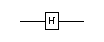
\includegraphics[scale=2]{Figures/circuits/H}};
\end{tikzpicture}
\caption{Clifford+T gates}
\label{fig:clifford}
\end{figure}

\begin{figure}
\vspace*{31mm}
\hspace*{72mm}
\begin{tikzpicture}[transform canvas={scale=0.8}]
  \node[font=\itshape\large] (textgg) {\(\forall g\in\{H,X,Y,Z\}\) cancels itself};
  \node[below=-5mm of textgg] (gg) {
    \begin{tikzpicture}
      \node[inner sep=0pt] (c1) at (0,0) {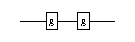
\includegraphics[scale=2]{Figures/circuits/gg}};  
      \node[right=-12mm of c1.east, rectangle, fill=white, minimum size=10mm] (eq) {\(=\)};    
      \node[right=-7mm of eq, inner sep=0pt] (c2) {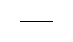
\includegraphics[scale=2]{Figures/circuits/I}};
      \node[right=7mm of c1.west, rectangle,fill=white,minimum size=5mm] {};
      %\node[below right=-1mm and -23mm of eq] (alg) {\small \(g\in\{H,X,Y,Z\}\)};
    \end{tikzpicture}
  };
  \node[above right=28mm and 13mm of textgg, font=\itshape\large] (textCNOT) {CNOT flip};
  \node [below=-5mm of textCNOT] (CNOT) {
    \begin{tikzpicture}
      \node[inner sep=0pt] (c1) at (0,0) {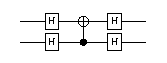
\includegraphics[scale=2]{Figures/circuits/HCNOTH}};       
      \node[right=-13.9mm of c1.east, inner sep=0pt] (c2) {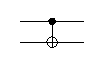
\includegraphics[scale=2]{Figures/circuits/CNOT}};
      \node[right=-12mm of c1.east, rectangle, fill=white, minimum size=10mm] (eq) {\(=\)};  
      \node[right=7mm of c1.west, rectangle,fill=white,minimum width=5mm, minimum height=10mm] {};
      \node[left=7mm of c2.east, rectangle,fill=white,minimum width=5mm, minimum height=10mm] {};
    \end{tikzpicture}
  };
  \node[above left=28mm and 0mm of textgg, font=\itshape\large] (textHXZ) {Rules with \(H\), \(X\), \(Y\) and \(Z\)};
  \node [below left=-5mm and -37mm of textHXZ] (XZ) {
    \begin{tikzpicture}
      \node[inner sep=0pt] (c1) at (0,0) {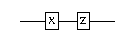
\includegraphics[scale=2]{Figures/circuits/XZ}};       
      \node[below=-3mm of c1] (eq) {\(=\)};  
      \node[below=-3mm of eq, inner sep=0pt] (c2) {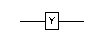
\includegraphics[scale=2]{Figures/circuits/Y}};
      \node[below=-3mm of c2] (eq2) {\(=\)};  
      \node[below=-3mm of eq2, inner sep=0pt] (c3) {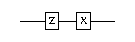
\includegraphics[scale=2]{Figures/circuits/ZX}};
      \node[right=7mm of c1.west, rectangle,fill=white,minimum size=5mm] {};
      \node[left=7mm of c3.east, rectangle,fill=white,minimum size=5mm] {};
      \node[left=7mm of c1.east, rectangle,fill=white,minimum size=5mm] {};
      \node[right=7mm of c3.west, rectangle,fill=white,minimum size=5mm] {};
    \end{tikzpicture}
  };
  \node [below right=-5mm and -37mm of textHXZ] (XH) {
    \begin{tikzpicture}
      \node[inner sep=0pt] (c1) at (0,0) {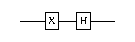
\includegraphics[scale=2]{Figures/circuits/XH}};       
      \node[below=-3mm of c1] (eq) {\(=\)};  
      \node[below=-3mm of eq, inner sep=0pt] (c2) {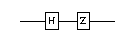
\includegraphics[scale=2]{Figures/circuits/HZ}};
      \node[right=7mm of c1.west, rectangle,fill=white,minimum size=5mm] {};
      \node[left=7mm of c2.east, rectangle,fill=white,minimum size=5mm] {};
      \node[left=7mm of c1.east, rectangle,fill=white,minimum size=5mm] {};
      \node[right=7mm of c2.west, rectangle,fill=white,minimum size=5mm] {};
    \end{tikzpicture}
  };  
  \node[below left=8mm and 7mm of textgg, font=\itshape\large] (textZS) {Rules with \(Z\), \(S\) and \(T\)};
  \node [below left=-5mm and -34mm of textZS] (ZS) {
    \begin{tikzpicture}
      \node[inner sep=0pt] (c1) at (0,0) {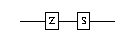
\includegraphics[scale=2]{Figures/circuits/ZS}};       
      \node[below=-3mm of c1] (eq) {\(=\)};  
      \node[below=-3mm of eq, inner sep=0pt] (c2) {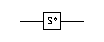
\includegraphics[scale=2]{Figures/circuits/S'}};
      \node[right=7mm of c1.west, rectangle,fill=white,minimum size=5mm] {};
      \node[left=7mm of c1.east, rectangle,fill=white,minimum size=5mm] {};
    \end{tikzpicture}
  };
  \node [below right=-5mm and -34mm of textZS] (ZT) {
    \begin{tikzpicture}
      \node[inner sep=0pt] (c1) at (0,0) {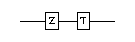
\includegraphics[scale=2]{Figures/circuits/ZT}};       
      \node[below=-3mm of c1] (eq) {\(=\)};  
      \node[below=-3mm of eq, inner sep=0pt] (c2) {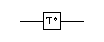
\includegraphics[scale=2]{Figures/circuits/T'}};
      \node[right=7mm of c1.west, rectangle,fill=white,minimum size=5mm] {};
      \node[left=7mm of c1.east, rectangle,fill=white,minimum size=5mm] {};
    \end{tikzpicture}
  };
  \node[below right=8mm and 3mm of textgg, font=\itshape\large] (textXS) {Rules with \(X\), \(S\) and \(T\)};
  \node [below left=-5mm and -34mm of textXS] (XS) {
    \begin{tikzpicture}
      \node[inner sep=0pt] (c1) at (0,0) {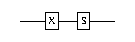
\includegraphics[scale=2]{Figures/circuits/XS}};       
      \node[below=-3mm of c1] (eq) {\(=\)};  
      \node[below=-3mm of eq, inner sep=0pt] (c2) {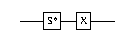
\includegraphics[scale=2]{Figures/circuits/SX}};
      \node[right=7mm of c1.west, rectangle,fill=white,minimum size=5mm] {};
      \node[left=7mm of c2.east, rectangle,fill=white,minimum size=5mm] {};
      \node[left=7mm of c1.east, rectangle,fill=white,minimum size=5mm] {};
      \node[right=7mm of c2.west, rectangle,fill=white,minimum size=5mm] {};
    \end{tikzpicture}
  };
  \node [below right=-5mm and -34mm of textXS] (XT) {
    \begin{tikzpicture}
      \node[inner sep=0pt] (c1) at (0,0) {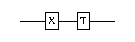
\includegraphics[scale=2]{Figures/circuits/XT}};       
      \node[below=-3mm of c1] (eq) {\(=\)};  
      \node[below=-3mm of eq, inner sep=0pt] (c2) {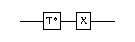
\includegraphics[scale=2]{Figures/circuits/TX}};
      \node[right=7mm of c1.west, rectangle,fill=white,minimum size=5mm] {};
      \node[left=7mm of c2.east, rectangle,fill=white,minimum size=5mm] {};
      \node[left=7mm of c1.east, rectangle,fill=white,minimum size=5mm] {};
      \node[right=7mm of c2.west, rectangle,fill=white,minimum size=5mm] {};
    \end{tikzpicture}
  };
\end{tikzpicture}
\vspace*{35mm}
\caption{Some basic properties of the gates in the Clifford+T set. Here, \(S^*\) and \(T^*\) represent the inverse gates of \(S\) and \(T\), i.e. their conjugate transpose, usually written as \(S^\dag\) and \(T^\dag\).}
\label{fig:props}
\end{figure}

The CNOT gate is particularly interesting. The qubit where the filled dot is (see Figure~\ref{fig:clifford}) acts as the `control', and the qubit with \(\oplus\) acts as the `target'. Whenever the control is \(\ket{0}\), no change is made in either of the qubits; but if it is \(\ket{1}\), an \(X\) gate is applied to the target, flipping the state of the qubit. This works in any superposition, so given an arbitrary two-qubit state \[\ket{c,t} = \alpha\ket{0,0} + \beta\ket{0,1} + \gamma\ket{1,0} + \delta\ket{1,1}\] if the CNOT were to act in \(\ket{c}\) as control and in \(\ket{t}\) as target, the outcome would be: \[CNOT \cdot \ket{c,t} = \alpha\ket{0,0} + \beta\ket{0,1} + \gamma\ket{1,1} + \delta\ket{1,0}\]

\textbf{MBQC model.} The acronym stand for Measurement Based Quantum Computing. Unlike the circuit model, where measurements are done at the very end of the circuit, MBQC carries out computations by means of repeatedly measuring an initially entangled resource. The process can be thought of as sculpting a rock. The rock would be the initial resource, which is a collection of entangled qubits forming certain lattice structure. By measuring some qubits in the lattice -- hitting the rock with a chisel -- we remove some of the excess qubits, changing the overall state in the process. The outcome of measurements is probabilistic so, in order to provide deterministic computation, we must apply corrections on the neighbouring qubits whenever the measurement outcome deviated from the desired result. After multiple iterations of measurements and corrections, we end up with a set of qubits encoding the result. In this model, the input is incorporated into the lattice at the beginning of the process.

In this way, any computation may be performed by applying 1-qubit measurements and 1-qubit correcting gates (controlled by classical signals). The initial resource state contains all the entanglement that is required, which may be prepared experimentally through multi-qubit interactions, such as Ising interactions~\citep{1WQC}, which are within our experimental capabilities. This model deals with the connectivity problem by applying a single operation involving \textit{all} the qubits at the beginning of the process, then only requiring cheap single qubit operations for the rest of the computation. The main drawback of MBQC is the large amount of qubits that are required for even the simplest of operations. The MBQC model was proposed for the first time by \citet{1WQC} under the name of \textit{one-way quantum computer}, which highlights its main difference with the circuit (reversible) approach. 

\textbf{Distributed model.} We may find a balance between the circuit model and MBQC. In it, multiple small quantum processing units (QPUs) would run fragments of the overall circuit. Communication is achieved through a shared entangled resource, reminiscent of the MBQC approach. This model has been discussed in detail in the literature~\citep{DistributedQCHW} and it is at the core of the main project from the Networked Quantum Information Technologies Hub (NQIT)\footnote{A project supported by the UK National Quantum Technology program, aiming to provide scalable quantum computing.}. In \S\ref{DQC_Architecture}, we discuss an abstract distributed quantum architecture in detail.



\section{Programming on quantum computers}

As of today, most quantum programming languages are merely high level circuit descriptors, providing the means to define circuits gate by gate, or build them up from combinations of smaller circuits. All of the well-known languages belong to this category, such as \textit{QCL}~\citep{QCL} (imperative paradigm, and one of the first quantum programming languages ever implemented), \textit{Q\#}~\citep{QLang} (imperative, designed by Microsoft), and \textit{Quipper}~\citep{Quipper} (functional, built on top of Haskell). 

Besides, there are attempts at designing quantum programming languages that are completely hardware agnostic, meaning they aim to describe the computation, rather than a particular circuit that implements it. Examples of these are the different attempts at defining a quantum lambda calculus, for instance the ones by \citet{VanTonder} or \citet{Diaz-Caro}. However, these are not particularly programmer friendly, as they are generally quite verbose.

Most of the literature on quantum algorithms describes them by explicitly giving a circuit that implements the algorithm. Fortunately, there is a constructive procedure, given by the Solovay-Kitaev theorem -- of which \citet{SolovayKitaev} give a good introductory review --, that takes any circuit and a choice of universal gate-set and outputs an efficient equivalent circuit using only those gates. Hence, programmers do not need to worry about the gates they are using when describing their circuits.

Unfortunately, the fact that algorithms are almost exclusively defined in the circuit model implies that other models of quantum computing are disregarded by a large portion of the community. In order to make other models of computation accessible, we need to provide automated procedures for transforming algorithms from the circuit model to the rest (and vice versa). Work has been done on the transformation from circuit to MBQC and backwards, the latter being the most challenging~\citep{gflow}. However, there is little amount of literature describing how to go from the circuit model to the distributed model. In \S\ref{IntroDistributing} we give an overview of the existent work on that aspect, and identify the gap on the literature we aim to cover in this thesis.

%\begin{mdframed}[backgroundcolor=gray!20,leftmargin=20pt,rightmargin=20pt, innerbottommargin=10pt] 
\begin{remark} \normalfont 
Here are the key concepts to keep in mind while reading the rest of this thesis:
\begin{itemize}
\item Quantum computers provide a computing power well beyond the capabilities of classical computers, which would be exploitable in many areas of science.
\item Small quantum computers are already available. 
\item Scaling up is a challenging problem due to: \textit{decoherence}, which may be overcome by the joint effort of the error-correction, physics and engineering communities; and \textit{connectivity}, which may be solved using distributed architectures.
\item There is practically no programming support for distributed architectures.
\end{itemize}
\end{remark}
%\end{mdframed}
\chapter{Distributed Quantum Computing}
\label{chap:Distributed}

As we discussed in \S\ref{Hardware}, there are different approaches on how to build quantum computers. Now that many of these have been experimentally demonstrated, the question of how to scale up is increasingly relevant. This has led to the proposal of distributed architectures~\citep{ArchitectureSurvey}.

In classical computing, an standard example of a distributed computer is the Non-Uniform Memory Access (NUMA) architecture: A system of independent computing nodes, each having its own local memory. In order to collaborate to perform an overall computation, the different nodes will need to communicate. In NUMA, they do so by accessing each other's memory. While nodes can manage their own local memory efficiently, accessing another node's memory is slow. Hence, we always attempt to minimise the amount of communication between nodes. A distributed quantum computer would follow the same principles, where each quantum processing unit (QPU) would own a collection of qubits (its local memory) and may access another QPU's qubits at the cost of some overhead, using entanglement.

\section{Communication through entanglement}
\label{Ebits}

For a QPU to be able to access another's qubit, we must provide them with some sort of communication channel. Simply using a classical channel (sending bits) is not helpful: the whole point of representing the state of the computation in qubits is that they may be in a superposition of classical states, which would take up to an exponential amount of space and processing on bits. We could consider physically moving the system that encodes the qubit from one QPU to another, and while that is certainly possible with photons, in general it is not feasible to have a channel that is both fast and protects well against information loss due to decoherence.

In \S\ref{Principles}, we explained it was possible to affect a distant qubit by acting on another qubit with which it was entangled. We wish to exploit this property in order to allow a QPU to query another's QPU qubits. There are different degrees of how strong a pair of qubits is entangled -- intuitively, how much they affect each other. This is often formalised as the correlation between the qubits measurement outcomes; for instance, the pair of qubits \(\frac{1}{\sqrt{2}}\ket{0,0} + \frac{1}{\sqrt{2}}\ket{1,1}\) is said to be \textit{maximally entangled}, as the possible measurement outcomes are exclusively either \(\ket{0,0}\) or \(\ket{1,1}\), always matching in both qubits. Naturally, the most efficient communication channel will take advantage of entanglement in its strongest form, and so we will make use pairs of qubits entangled in this particular maximally entangled state. This qubit pair configuration is generally known as a Bell state, and Figure~\ref{fig:bell} shows how to prepare it.

\begin{figure}
  \hspace*{20mm}
  \begin{tikzpicture}
    \node[inner sep=0pt] (circuit) at (0,0) {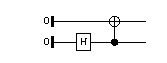
\includegraphics[scale=2]{Figures/circuits/Bell}};
    \node[right=8mm of circuit.north west, font=\itshape] (text) {a)};
  \end{tikzpicture} 
  \begin{tikzpicture}
    \node[inner sep=0pt] (circuit) at (0,0) {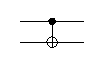
\includegraphics[scale=2, trim={5mm 0 0 0},clip]{Figures/circuits/CNOT}};
    \node[rectangle, fill=white, minimum size=5mm] (clear) at (-5mm,-5mm) {};
    \pic (e1) {ebit=e1/5.63mm/13mm};
    \node[right=2mm of circuit.north west, font=\itshape] (text) {b)};
  \end{tikzpicture}
\caption{Generation of the Bell state \(\ket{\Phi^+} = \frac{1}{\sqrt{2}}\ket{0,0} + \frac{1}{\sqrt{2}}\ket{1,1}\) shown in \textit{a)}. Its shorthand circuit notation is given in \textit{b)}.}
\label{fig:bell}
\end{figure}

An interesting property of the Bell state is shown in Figure~\ref{fig:sliding}: if a quantum gate, whose matrix representation is symmetric, is applied to one of the qubits, it is the same as if the gate was applied to the other qubit. In some sense, the gate can `slide' through the entanglement, like beads on a string; as if the entangled state were a curved wire, connecting the pair of qubits. Hopefully, this serves as a first intuition of how Bell states are a natural choice for implementing quantum comunication.

\begin{figure}
  \hspace*{30mm}
  \begin{tikzpicture}
    \node[inner sep=0pt] (circuit) at (0,0) {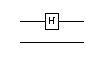
\includegraphics[scale=2, trim={0 0 5mm 0},clip]{Figures/circuits/H_I}};
    \pic (e1) {ebit=e1/5.63mm/13mm};
    \node[right=2mm of circuit.north west, font=\itshape] (text) {a)};
  \end{tikzpicture} 
  \hspace*{10mm}
  \begin{tikzpicture}
    \node[inner sep=0pt] (circuit) at (0,0) {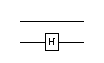
\includegraphics[scale=2, trim={0 0 5mm 0},clip]{Figures/circuits/I_H}};
    \pic (e1) {ebit=e1/5.63mm/13mm};
    \node[right=2mm of circuit.north west, font=\itshape] (text) {b)};
  \end{tikzpicture}
\caption{Applying a gate on a Bell state. The circuits shown in \textit{a)} and \textit{b)} are equivalent.}
\label{fig:sliding}
\end{figure}

\subsection{Entanglement distillation}
\label{Distillation}

So far, we have explained how to generate a Bell state \(\ket{\Phi^+} = \frac{1}{\sqrt{2}}\ket{0,0} + \frac{1}{\sqrt{2}}\ket{1,1}\) inside a QPU (as in Figure~\ref{fig:bell}). However, what we aim for is that two different QPUs each own one of the qubits from \(\ket{\Phi^+}\). The challenge is then to send one of the qubits to another QPU, while preserving the state. The problem of sharing a Bell state between two parties is solved by the \textit{entanglement distillation} protocol~\citep{DistillationProtocol}, which ensures the shared pair of qubits are in the Bell state, up to some small error factor. In this section, we will give a brief explanation of how this protocol works.

In practice, there are no perfect communication channels. This means that it is impossible to send a quantum state without potentially altering it, introducing errors. And, as we mentioned earlier in \S\ref{Challenges}, detecting and correcting errors in quantum information is particularly challenging. Fortunately, in our case there is an easy way around it. We can create multiple \(\ket{\Phi^+}\) states in the first QPU, and send one of the qubits of each of these pairs to the second QPU, through a noisy channel. Then, we would have shared multiple imperfect \(\ket{\Phi^+}\) pairs, whose fidelity we can improve by making them interact with each other, destroying some of the pairs in the process. Before going into details on how we perform these interactions, we need some definitions:

\begin{itemize}
  \item \textit{Werner state}: It is the result of sending one of the qubits from \(\ket{\Phi^+}\) through a noisy channel characterised by a constant \(F \in [0,1]\). \(F\) determines the \textit{fidelity} of the channel, i.e.\ the probability that the qubit is sent without altering its state. Rather than an actual quantum state, the Werner state is a probability distribution of quantum states, known in the literature as a \textit{mixed state}. In particular, it is the probability distribution of actually having \(\ket{\Phi^+}\), with probability \(F\), or having \(\ket{\Phi^+}\) with an \(X\) gate mistakenly applied to the sent qubit, having \(\ket{\Phi^+}\) with a \(Z\) gate on it or having \(\ket{\Phi^+}\) with both \(X\) and \(Z\) errors, each of these three cases\footnote{Although a channel will rarely introduce each of these errors with equal \(\frac{1-F}{3}\) probability, it is always possible to apply some local operations on each of the qubits so the probability distribution converges to that of the Werner state. Moreover, there may be channels that introduce errors other than \(X\) and \(Z\); however the resulting state after sharing \(\ket{\Phi^+}\) through any of these will always be some Werner state with some particular \(F\).} occurring with equal probability \(\frac{1-F}{3}\).

  \item \textit{Bilateral XOR (BXOR)}: Simply, two CNOT gates applied inside two different QPUs. Its intended use is to be applied to two Werner states; one QPU should have one of the qubits of each Werner state, and apply a CNOT on them, while the other should do the same on the other two qubits. Thus, one of the Werner states acts as control of both CNOTs, and the other as their target.
\end{itemize}

The entanglement distillation protocol takes a collection of Werner states and repeats the following three steps multiple times, until the fidelity of the Werner states is the one desired:

\begin{enumerate}
  \item Make pairs of two Werner states, and apply a BXOR to each pair. The new probability distribution (mixed state) on each of these four qubits is given in Table~\ref{tab:Werners}.

  \item For each pair of Werner states, measure the qubits corresponding to the Werner state that acted as the target of the BXOR -- this will require one measurement in each QPU. The outcome of the two measurements will match precisely in the cases where the fifth column of Table~\ref{tab:Werners} shows no \(X\) error. Examining the table, we can calculate the probability of that event: {\small \[T(F) = F^2 + \frac{2}{3} F(1-F) + \frac{5}{9} (1-F)^2\]}which, for \(F > \frac{1}{2}\), is always over a half.

  \item If the outcome of both measurements matched, keep the other two qubits (i.e.\ the control Werner state). Otherwise, discard them, not to be used again. Among the eight cases when we keep the Werner state, in two of them (grayed rows in Table~\ref{tab:Werners}) the state we keep has no errors. This happens with probability: {\small \[P(F) = \frac{F^2 + 1/9(1-F)^2}{T(F)}\]}Thus, the kept qubit pairs are all Werner states with fidelity \(P(F)\) which, as shown in Figure~\ref{fig:fidelity}, is greater than \(F\) whenever \(F > \frac{1}{2}\).
\end{enumerate}

\begin{table}
\caption{Probability distribution defining a pair of Werner states, and the errors present in each case, before and after the BXOR is applied.}
\label{tab:Werners}
\scriptsize
\centering
\begin{tabular}{|c|cc|cc|c|}
\hline
\multicolumn{1}{|c|}{\multirow{2}{*}{Probability}} & \multicolumn{2}{c|}{Errors before} & \multicolumn{2}{c|}{Errors after} & \multicolumn{1}{c|}{\multirow{2}{*}{Kept?}} \\
\multicolumn{1}{|c|}{} & {\tiny Source} & {\tiny Target} & {\tiny Source} & {\tiny Target} & \multicolumn{1}{c|}{} \\
\hline
\rowcolor{gray!30}
\(F^2\) & -- & -- & -- & -- & \cmark \\ %THIS
\(\frac{1}{3}F(1-F)\) & -- & \(Z\) & \(Z\) & \(Z\) & \cmark \\
\(\frac{1}{3}F(1-F)\) & -- & \(X\) & -- & \(X\) & \\
\(\frac{1}{3}F(1-F)\) & -- & \(X,Z\) & \(Z\) & \(X,Z\) & \\
\(\frac{1}{3}F(1-F)\) & \(Z\) & -- & \(Z\) & -- & \cmark \\
\rowcolor{gray!30}
\(\frac{1}{9}(1-F)^2\) & \(Z\) & \(Z\) & -- & \(Z\) & \cmark \\ %THIS
\(\frac{1}{9}(1-F)^2\) & \(Z\) & \(X\) & \(Z\) & \(X\) & \\
\(\frac{1}{9}(1-F)^2\) & \(Z\) & \(X,Z\) & -- & \(X,Z\) & \\ 
\hline
\end{tabular}
\hspace{10pt}
\begin{tabular}{|c|cc|cc|c|}
\hline
\multicolumn{1}{|c|}{\multirow{2}{*}{Probability}} & \multicolumn{2}{c|}{Errors before} & \multicolumn{2}{c|}{Errors after} & \multicolumn{1}{c|}{\multirow{2}{*}{Kept?}} \\
\multicolumn{1}{|c|}{} & {\tiny Source} & {\tiny Target} & {\tiny Source} & {\tiny Target} & \multicolumn{1}{c|}{} \\
\hline
\(\frac{1}{3}F(1-F)\) & \(X\) & -- & \(X\) & \(X\) & \\
\(\frac{1}{9}(1-F)^2\) & \(X\) & \(Z\) & \(X,Z\) & \(X,Z\) & \\
\(\frac{1}{9}(1-F)^2\) & \(X\) & \(X\) & \(X\) & -- & \cmark \\
\(\frac{1}{9}(1-F)^2\) & \(X\) & \(X,Z\) & \(X,Z\) & \(Z\) & \cmark \\
\(\frac{1}{3}F(1-F)\) & \(X,Z\) & -- & \(X,Z\) & \(X\) & \\
\(\frac{1}{9}(1-F)^2\) & \(X,Z\) & \(Z\) & \(X\) & \(X,Z\) & \\
\(\frac{1}{9}(1-F)^2\) & \(X,Z\) & \(X\) & \(X,Z\) & -- & \cmark \\
\(\frac{1}{9}(1-F)^2\) & \(X,Z\) & \(X,Z\) & \(X\) & \(Z\) & \cmark \\
\hline
\end{tabular}
\end{table}

\begin{figure}
\caption{Fidelity after a single iteration of the distillation protocol, versus the original fidelity. The figure shows that \(F > \frac{1}{2} \, \Rightarrow \, P(F) > F\).}
\label{fig:fidelity}
\centering
\begin{tikzpicture}
\begin{axis}[
    axis lines = left,
    xlabel = $F$,
    ylabel = {$P(F)$},     
    no markers,
    every axis plot/.append style={thick},
    every x tick label/.append style={font=\scriptsize},
    every y tick label/.append style={font=\scriptsize}]
\addplot[domain=0:1, samples=100, color=black!95]{(1 - x)^2/9 + x^2)/((5*(1 - x)^2)/9 + (2*(1 - x)*x)/3 + x^2};
\addplot[domain=0:1, samples=3, color=black!70, style=dashed]{x};
\end{axis}
\end{tikzpicture}
\end{figure}

Figure~\ref{fig:fidelity} implies that we may use a communication channel as noisy as to introduce errors slightly less than half of the times, and still generate a Werner state whose fidelity is arbitrarily close to one. Naturally, the more fidelity we wish to attain, and the worse the fidelity we start with is, more iterations of the protocol will be required. This would increase the amount of time and resources -- number of initial Werner states -- we must pay in order to obtain a single entangled qubit pair.

Often in distributed quantum computing literature, a Bell state shared by two QPUs is known as an \textit{ebit} (entangled-bit) which, put another way, is just a Werner state with a fidelity close to one. Thus, this protocol produces ebits, which is the fundamental resource for quantum communication in distributed circuits. During the rest of this thesis, we use the term \textit{ebit half} to refer to any of the two qubits that comprise an ebit.

\section{Distributing circuits}
\label{IntroDistributing}

We now explain how ebits are used to allow a QPU to peek into another's qubits. Here, we will introduce the proposal of \citet{NonLocalCNOT}. Later on, in \S\ref{NonLocalGates}, we will extend this work with our own contributions. 

We aim to split a given circuit and distribute the fragments across multiple QPUs. The gates that should operate over qubits on different QPUs are known as \textit{non-local} gates. As we previously mentioned in \S\ref{Models}, any circuit can be converted to Clifford+T circuit. In Clifford+T, the only gate that operates on more than one qubit is the CNOT. Hence, we only need to understand how CNOTs can be implemented non-locally.

The construction we will use is a slight variation of what was proposed by \citet{NonLocalCNOT}, and its scheme is shown in Figure~\ref{fig:nonlocalCNOT}. In principle, we will use an \textit{ebit} per non-local CNOT. We will call the QPU that holds the target qubit (the one with a \(\oplus\)) the `target QPU' and similarly for the control qubit. 

\begin{figure}
\begin{tikzpicture}
  \node[inner sep=0pt] (circuit) at (0,0) {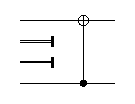
\includegraphics[scale=2,trim={10mm 0 5mm 0},clip]{Figures/circuits/cnotToCut}};
  \coordinate[left=1mm of circuit.west] (leftPoint);
  \coordinate[right=1mm of circuit.east] (rightPoint);
  \pic (cut) {cut=leftPoint/rightPoint};
  \node[left=-2mm of circuit.north west, font=\itshape] (text) {a)};
  \node[font=\scriptsize\itshape, opacity=0.9, above right=3mm and -4mm of leftPoint] (QPUA) {QPU A};
  \node[font=\scriptsize\itshape, opacity=0.9, below right=3mm and -4mm of leftPoint] (QPUB) {QPU B};
\end{tikzpicture}
\hspace{3mm}
\begin{tikzpicture}
  \node[inner sep=0pt] (circuit) at (0,0) {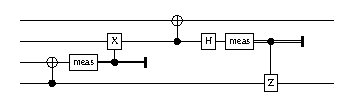
\includegraphics[scale=2]{Figures/circuits/nonlocalCNOT}};
  \pic (e1) {ebit=e1/12.7mm/13mm};
  \coordinate[left=-5.5mm of circuit.west] (leftPoint);
  \coordinate[right=-5.5mm of circuit.east] (rightPoint);
  \pic (cut) {cut=leftPoint/rightPoint};
  \pic [below left=27mm and -13mm of circuit.north west] (entangler) {opaquebox=entangler/9mm/55mm/23mm/41mm/cat-entangler};
  \pic [below left=27mm and -13mm of circuit.north west] (disentangler) {opaquebox=disentangler/9mm/105mm/23mm/39.5mm/cat-disentangler};
  \node[right=2mm of circuit.north west, font=\itshape] (text) {b)};
  \node[font=\scriptsize\itshape, opacity=0.9, above right=3mm and -4mm of leftPoint] (QPUA) {QPU A};
  \node[font=\scriptsize\itshape, opacity=0.9, below right=3mm and -4mm of leftPoint] (QPUB) {QPU B};
\end{tikzpicture}
\caption
{A non-local CNOT, shown in \textit{a)}. The dashed line indicates how the circuit is separated into two QPUs. The implementation scheme is given in \textit{b)}.}
\label{fig:nonlocalCNOT}
\end{figure}

The implementation of a non-local CNOT gate has three steps. First, we must apply what the authors refer to as the \textit{cat-entangler} (shown in Figure~\ref{fig:cat-entangler}), which creates a local `copy'\footnote{Note that there is no such thing as copying a quantum state (due to the non-cloning theorem). What we mean here by `copying' is generating, from \(\ket{\psi} = \alpha\ket{0} + \beta\ket{1}\), the state \(\ket{\psi'} = \alpha\ket{0,0} + \beta\ket{1,1}\) where each of the classical states is duplicated. This is fundamentally different from an actual copy: \(\ket{\psi}\otimes\ket{\psi} = \alpha^2\ket{0,0} + \alpha\beta\ket{0,1} + \alpha\beta\ket{1,0} + \beta^2\ket{1,1}\).} of the control qubit inside the target QPU. In the process, the ebit half in the control QPU is measured (and thus destroyed), and the outcome is used to correct the other half, in the same spirit as in the MBQC model. These corrections are done via \textit{classically controlled gates}; devices that either apply a transformation to the qubit or none, depending on the value of a classical bit. Notice that the only information physically crossing the boundary between blocks is the \textit{classical} outcome of the measurement (a bit, either \(0\) or \(1\)).

\begin{figure}
\centering
\begin{tikzpicture}
  \node[inner sep=0pt] (circuit) at (0,0) {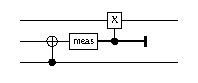
\includegraphics[scale=2]{Figures/circuits/entangler}};
  \pic (e1) {ebit=e1/5.63mm/13mm};
  \coordinate[below left=10.7mm and 0mm of circuit.north west] (leftPoint);
  \coordinate[right=61mm of leftPoint] (rightPoint);
  \pic (cut) {cut=leftPoint/rightPoint};
  \node[font=\scriptsize\itshape, opacity=0.9, above right=3mm and -3mm of leftPoint] (QPUA) {QPU A};
  \node[font=\scriptsize\itshape, opacity=0.9, below right=3mm and -3mm of leftPoint] (QPUB) {QPU B};
\end{tikzpicture}
\caption{Implementation of the cat-entangler. An ebit is used to make the information in QPU \(B\)'s wire available to QPU \(A\). A doubled line indicates the wire holds classical information. Hence, the \(X\) gate is classically controlled, and the line that crosses the boundary represents classical communication. For any input state \(\alpha\ket{0} + \beta\ket{1}\), the output is \(\alpha\ket{0,0} + \beta\ket{1,1}\).}
\label{fig:cat-entangler}
\end{figure}

Then, the CNOT gate is applied \textit{locally} inside the target QPU, between its ebit half and the target qubit. At the end, the \textit{cat-disentangler} must be applied (shown in Figure~\ref{fig:cat-disentangler}), which simply destroys -- with a measurement -- the remaining ebit half and then corrects the control qubit. Once again, only classical information crosses the boundary.

\begin{figure}
\centering
\begin{tikzpicture}
  \node[inner sep=0pt] (circuit) at (0,0) {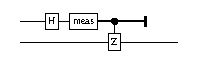
\includegraphics[scale=2]{Figures/circuits/disentangler}};
  \coordinate[below left=10.7mm and 0mm of circuit.north west] (leftPoint);
  \coordinate[right=61mm of leftPoint] (rightPoint);
  \pic (cut) {cut=leftPoint/rightPoint};
  \node[font=\scriptsize\itshape, opacity=0.9, above right=3mm and -3mm of leftPoint] (QPUA) {QPU A};
  \node[font=\scriptsize\itshape, opacity=0.9, below right=3mm and -3mm of leftPoint] (QPUB) {QPU B};
\end{tikzpicture}
\caption{Implementation of the cat-disentangler. Essentially, it destroys the ebit half (top wire) that the cat-entangler coupled with QPU B's wire. A doubled line indicates the wire holds classical information (a bit). For any input state \(\alpha\ket{0,0} + \beta\ket{1,1}\), the output is \(\alpha\ket{0} + \beta\ket{1}\).}
\label{fig:cat-disentangler}
\end{figure}

In this way, we have implemented a non-local CNOT gate using one ebit and two classical bit messages between QPUs. However, the true advantage of this approach is gained when multiple non-local CNOTs are implemented using a single ebit: Once the cat-entangler is applied, any number of CNOTs that are controlled by the same wire and whose target QPU is the same, may all be implemented using the same ebit half as control, as shown in Figure~\ref{fig:nonlocalCNOTs}.

\begin{figure}
\centering
\begin{tikzpicture}
  \node[inner sep=0pt] (circuit) at (0,0) {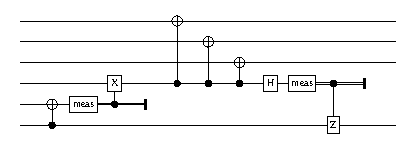
\includegraphics[scale=2]{Figures/circuits/nonlocalCNOTs}};
  \pic (e1) {ebit=e1/26.79mm/13mm};
  \pic [below left=27mm and -13mm of circuit.north west] (entangler) {box=entangler/23.5mm/52mm/23mm/38mm/Entangler/0mm/1mm};
  \pic [below left=27mm and -13mm of circuit.north west] (disentangler) {box=disentangler/23.5mm/126mm/23mm/38.5mm/Disentangler/10.5mm/1mm};
  \coordinate[below left=7mm and -6mm of circuit.west] (leftPoint);
  \coordinate[right=130.5mm of leftPoint] (rightPoint);
  \pic (cut) {cut=leftPoint/rightPoint};
\end{tikzpicture}
\caption{Implementing multiple non-local CNOTs using a single ebit. The bottom-most wire acts as control for the three of them. Only classical information crosses the boundary between QPUs.}
\label{fig:nonlocalCNOTs}
\end{figure}

Now, depending of how we choose to partition the circuit, there will be different groups of CNOTs that we may be able to implement using a single ebit. We will then wish to find the partition that requires the fewest ebits to implement all of its CNOT gates. This optimization problem is not discussed in the original paper, nor in any other work, as far as we know. It will be our main contribution in this thesis, along with an extension of the results just explained, both found in Chapter~\ref{chap:Project}.


\section{Distributed quantum architectures}
\label{DQC_Architecture} 

In this section we propose an abstract distributed quantum architecture. We claim that any distributed quantum computing technology will be characterised by the following features:

\begin{itemize}
  \item \textit{Multiple quantum processing units (QPUs)}: Each of the QPUs should be able to perform universal quantum computation on its collection of `workspace' qubits. It should be possible to prepare these qubits to hold the input data of a program, and read output from them (measurement). It should also be possible to apply classically controlled gates on the qubits.

  \item \textit{Specialised space for ebits}: Each QPU should have some extra qubits meant to be used as ebit halves. These should be specialised so the operations necessary for ebit generation can be applied on them fast and reliably. The QPU should support the application of CNOTs (or some other suitable 2-qubit gate) between these specialised qubits and the ones in its workspace.
  
  \item \textit{Ebit generation hardware}: This includes the (noisy) quantum communication channel itself and the ability to perform the distilling process. The generation of ebits may be done either in a centralised manner, with a separated device that creates Bell states and sends them to the different QPUs, or decentralised, each QPU having their own hardware for creating and sharing ebits. Depending on the technology used, entanglement distillation may be more or less essential; for instance, if the step of sharing Bell states is done using quantum optics (photons), the quantum channel is likely to be fairly reliable, so it would only require a few iterations of the distilling process.
  
  \item \textit{Classical communication network}: Which will be required in the process of entanglement distillation, as well as to perform cat-entanglers and cat-disentanglers. The QPUs will send signals through the network when they measure their qubits, and read from it to apply corrections. 
\end{itemize}

As we discussed in \S\ref{Distillation}, there is a compromise between the quality of the ebits and the effort put into preparing them. Fortunately, \citet{NoisyChannels} showed that efficient distributed quantum computation using noisy ebits is feasible. Nevertheless, ebit generation will always be the main bottle-neck of any distributed quantum architecture, as it is by far more expensive than classical communication and any local operation (in fact, multiple local operations are required in order to generate and use an ebit). Therefore, we will want to minimise the number of ebits required to implement any given algorithm.

\citet{DistributedQCHW} have proposed an experimental distributed quantum architecture. They explain how each of the features listed above may be implemented, particularly focusing on how entanglement across QPUs is achieved (ebit generation). Their proposal is to use cavities (traps) where the particles encoding the qubits are kept, and use laser pulses (photons) to entangle cavities of different QPUs together.
\chapter{Automated Distribution of Quantum Algorithms}
\label{chap:Project}

\section{Implementing non-local CNOT gates}
\label{NonLocalGates}

In \S\ref{IntroDistributing}, we explained the proposal by~\citet{NonLocalCNOT} of how to implement a non-local gate. We will now extend their results.

In the original work, in order to implement multiple non-local gates using a single ebit, there must not be any operation on the control qubit between the non-local gates. However, many of the 1-qubit gates from the Clifford+T set commute with the CNOT gate. This means that, if there are operations in between CNOTs, we may transform the circuit to an equivalent version where the CNOT gates are brought together. And although some of the gates do not commute with CNOT, in some cases they can still be interchanged with it if an additional 1-qubit gate is added. All of the relevant circuit transformations are shown in Figure~\ref{fig:pullRules}. These can be checked by calculating the corresponding matrices of both sides and verifying they match.

\begin{figure}
\hspace*{-6mm}
\begin{tikzpicture}
  \node[font=\itshape] (textA) {\(\forall g\in\{Z,S,T\}\) at control wire};
  \node [below=-5mm of textA] (A) {
    \begin{tikzpicture}
      \node[inner sep=0pt] (c1) at (0,0) {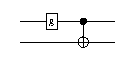
\includegraphics[scale=2]{Figures/circuits/C_gCNOT}};       
      \node[right=-13.9mm of c1.east, inner sep=0pt] (c2) {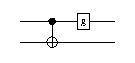
\includegraphics[scale=2]{Figures/circuits/C_CNOTg}};
      \node[right=-12mm of c1.east, rectangle, fill=white, minimum size=10mm] (eq) {\(=\)};  
      \node[right=7mm of c1.west, rectangle,fill=white,minimum width=5mm, minimum height=10mm] {};
      \node[left=7mm of c2.east, rectangle,fill=white,minimum width=5mm, minimum height=10mm] {};
    \end{tikzpicture}
  };
  \node[right=20mm of textA, font=\itshape] (textB) {\(\forall g\!\text{'}\in\{X,Y\}\) at control wire};
  \node [below=-5mm of textB] (B) {
    \begin{tikzpicture}
      \node[inner sep=0pt] (c1) at (0,0) {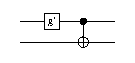
\includegraphics[scale=2]{Figures/circuits/C_g2CNOT}};       
      \node[right=-13.9mm of c1.east, inner sep=0pt] (c2) {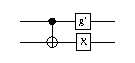
\includegraphics[scale=2]{Figures/circuits/C_CNOTg2}};
      \node[right=-12mm of c1.east, rectangle, fill=white, minimum size=10mm] (eq) {\(=\)};  
      \node[right=7mm of c1.west, rectangle,fill=white,minimum width=5mm, minimum height=10mm] {};
      \node[left=7mm of c2.east, rectangle,fill=white,minimum width=5mm, minimum height=10mm] {};
    \end{tikzpicture}
  };
  \node[below=20mm of textA, font=\itshape] (textC) {\(\forall g\in\{X\}\) at target wire};
  \node [below=-5mm of textC] (C) {
    \begin{tikzpicture}
      \node[inner sep=0pt] (c1) at (0,0) {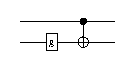
\includegraphics[scale=2]{Figures/circuits/T_gCNOT}};       
      \node[right=-13.9mm of c1.east, inner sep=0pt] (c2) {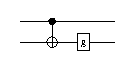
\includegraphics[scale=2]{Figures/circuits/T_CNOTg}};
      \node[right=-12mm of c1.east, rectangle, fill=white, minimum size=10mm] (eq) {\(=\)};  
      \node[right=7mm of c1.west, rectangle,fill=white,minimum width=5mm, minimum height=10mm] {};
      \node[left=7mm of c2.east, rectangle,fill=white,minimum width=5mm, minimum height=10mm] {};
    \end{tikzpicture}
  };
  \node[below=20mm of textB, font=\itshape] (textD) {\(\forall g\!\text{'}\in\{Y,Z\}\) at target wire};
  \node [below=-5mm of textD] (D) {
    \begin{tikzpicture}
      \node[inner sep=0pt] (c1) at (0,0) {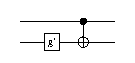
\includegraphics[scale=2]{Figures/circuits/T_g2CNOT}};       
      \node[right=-13.9mm of c1.east, inner sep=0pt] (c2) {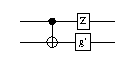
\includegraphics[scale=2]{Figures/circuits/T_CNOTg2}};
      \node[right=-12mm of c1.east, rectangle, fill=white, minimum size=10mm] (eq) {\(=\)};  
      \node[right=7mm of c1.west, rectangle,fill=white,minimum width=5mm, minimum height=10mm] {};
      \node[left=7mm of c2.east, rectangle,fill=white,minimum width=5mm, minimum height=10mm] {};
    \end{tikzpicture}
  };
\end{tikzpicture}
\caption{Different cases when a 1-qubit gate from Clifford+$T$ can be pushed through a CNOT gate.}
\label{fig:pullRules}
\end{figure}

The second improvement comes by realising that the method used to implement multiple CNOT gates controlled by the same wire (explained in \S\ref{IntroDistributing}) can also be applied if multiple CNOT have a common target qubit instead. We will refer to the former method as the \textit{remote-control} method and \textit{remote-target} for the latter. The derivation of the remote-target method is shown in Figure~\ref{fig:CNOTtargetProof}, which uses some of the properties listed in \S\ref{Models}. The main difference is that the CNOT itself is now applied in the control QPU instead of the target, so the cat-entangler and cat-disentangler must change accordingly.

\begin{figure}
\vspace*{11mm}
\hspace*{73mm}
\begin{tikzpicture}[transform canvas={scale=0.73}]
  \node (A) {
    \begin{tikzpicture}
      \node[inner sep=0pt] (c1) {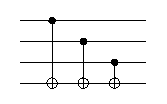
\includegraphics[scale=2]{Figures/circuits/proof1}};  
      \coordinate[below left=7mm and -6mm of c1.west] (l1);
      \coordinate[right=45mm of l1] (r1);
      \pic (cut1) {cut=l1/r1};     
      \node[right=0mm of c1] (eq1) {\Large \(=\)}; 
      \node[right=0mm of eq1, inner sep=0pt] (c2) {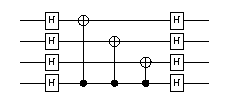
\includegraphics[scale=2]{Figures/circuits/proof2}};  
      \coordinate[below left=7mm and -6mm of c2.west] (l2);
      \coordinate[right=66mm of l2] (r2);
      \pic (cut2) {cut=l2/r2};  
      \node[right=0mm of c2] (eq2) {\Large \(=\)};  
    \end{tikzpicture}
  };
  \node[below=5mm of A] (B) {
    \begin{tikzpicture}
      \node (eq2) {\Large \(=\)};    
      \node[right=-4mm of eq2, inner sep=0pt] (circuit) {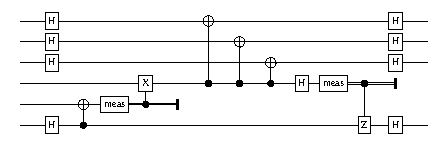
\includegraphics[scale=2]{Figures/circuits/proof3}};  
      \pic (e3) {ebit=e3/26.79mm/13mm};  
      \coordinate[below left=7mm and -6mm of circuit.west] (l3);
      \coordinate[right=140mm of l3] (r3);
      \pic (cut3) {cut=l3/r3};  
      \node[right=0mm of circuit] (eq3) {\Large \(=\)}; 
    \end{tikzpicture}
  };
  \node[below=5mm of B] (C) {
    \begin{tikzpicture}
      \node (eq3) {\Large \(=\)}; 
      \node[right=0mm of eq3, inner sep=0pt] (circuit) {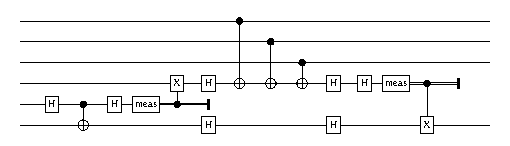
\includegraphics[scale=2]{Figures/circuits/proof4}};   
      \pic (e4) {ebit=e4/26.79mm/13mm};  
      \coordinate[below left=7mm and -6mm of circuit.west] (l4);
      \coordinate[right=161mm of l4] (r4);
      \pic (cut4) {cut=l4/r4};  
      \node[right=0mm of circuit] (eq4) {\Large \(=\)}; 
    \end{tikzpicture}
  };
  \node[below=5mm of C] (D) {
    \begin{tikzpicture}
      \node (eq4) {\Large \(=\)};    
      \node[right=-4mm of eq4, inner sep=0pt] (circuit) {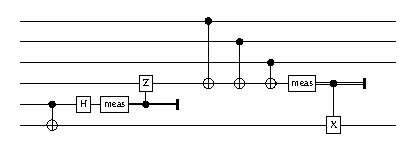
\includegraphics[scale=2]{Figures/circuits/proof5}};     
      \pic (e5) {ebit=e5/26.79mm/13mm};  
      \coordinate[below left=7mm and -6mm of circuit.west] (l5);
      \coordinate[right=129mm of l5] (r5);
      \pic (cut5) {cut=l5/r5};  
      \node[right=-4mm of circuit] (eq5) {\Large \(=\)};    
      \node[right=-4mm of eq5, inner sep=0pt] (c6) {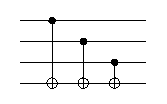
\includegraphics[scale=2]{Figures/circuits/proof1}};   
      \coordinate[below left=7mm and -6mm of c6.west] (l6);
      \coordinate[right=45mm of l6] (r6);
      \pic (cut6) {cut=l6/r6};  
    \end{tikzpicture}
  };
\end{tikzpicture}
\vspace*{140mm}
\caption{Proof of the implementation of multiple non-local CNOT gates that share a common target. The proof uses properties given in Figures~\ref{fig:props}, \ref{fig:sliding} and~\ref{fig:nonlocalCNOTs}. The distributed circuit is similar to the case for share control (Figure~\ref{fig:nonlocalCNOTs}). Both cat-entangler and cat-disentangler slightly differ.}
\label{fig:CNOTtargetProof}
\end{figure}

\section{Finding an efficient distribution}
\label{EfficientDistrib}

In this section we explain how we search for a suitable distribution of the circuit. But first, we establish what we mean by a distributed circuit to be efficient. This is based on what was discussed in \S\ref{DQC_Architecture} to be the bottle-necks of a distributed quantum architecture. A distributed circuit is efficient when there is:

\begin{itemize}
  \item \textit{Minimal amount of quantum communication} between the QPUs, meaning it requires as little number of ebits as possible. In comparison, message passing of classical bits is considered negligible and it is not taken into account.
  \item \textit{Load-balance across the QPUs}, up to a tolerance margin. Our notion of load-balance is that the different QPUs have a similar number of qubits assigned to them. A uniform depth of the local circuits (i.e.\ length of the circuits) would be desirable. However, the distributed circuit depth is inherited from the original circuit, as none of our distribution techniques change the depth in a significant way. Hence, we will not take circuit depth into account, and instead assume that already known methods for depth reduction, such as the one described by~\citet{DepthReduction}, have already been applied on the input circuit, and may be applied again to each QPU's local circuit. As circuit depth is not something we aim to optimise, we consider the cost of local gates negligible.
\end{itemize}

The problem at hand is similar to the  \textit{(\(k,\varepsilon\))-graph partitioning} problem. In it, a graph partition in \(k\) subgraphs has to be found, minimising the number of \textit{cut edges}: edges that have their incident vertices in different subgraphs. Additionally, the resulting partition must satisfy that the number of vertices in each subgraph is less than \((1 \pm \varepsilon)\frac{N}{k}\), where \(N\) is the total number of vertices in the graph. In Table~\ref{tab:matching} we list the correspondences between these two problems.

\begin{table}
\caption{Correspondence between the graph partitioning problem and the efficient distribution of quantum circuits.}
\label{tab:matching}
\centering
\begin{tabular}{|c|c|}
\hline
\textit{Graph partitioning} & \textit{Efficient distribution} \\
\hline
Vertices & Circuit wires \\
Edges & CNOT gates \\
Partitioned graph & Distributed circuit \\
Subgraph & QPU \\
Min. cut edges & Min. non-local gates \\
Uniform subgraph size & Load-balance \\
\hline
\end{tabular}
\end{table}

But there is a caveat. If we use graph partitioning naively, we will not be exploiting the fact that multiple CNOT gates may be implemented using a single ebit. In what follows, we will explain how to make use of \textit{hypergraph} partitioning, instead of simple graph partitioning, to account for this aspect. A more detailed review of the hypergraph partition problem is given in Appendix~\ref{chap:HypPart}, here we summarise the key concepts:

\begin{itemize}
  \item Hypergraphs extend graphs to accommodate edges that may have more than two incident vertices. More formally, a hypergraph is a pair \((V,H)\), where \(V\) is the set of vertices and \(H \subseteq 2^V\) is the collection\footnote{\, We will allow multiple hyperedges connecting the same vertices, in the same way as multigraphs allow multiple edges across any pair of edges.} of hyperedges. Each hyperedge is represented as the subset of vertices from \(V\) it connects. We will not consider any notion of directionality.
  \item Hypergraph partitioning follows the same premise as graph partitioning. The user provides a hypergraph and two parameters \((k,\varepsilon)\), which have the exact same meaning as before. What the problem now attempts to minimise is a metric known as \(\lambda\!-\!1\), which is defined as follows: Given a partition of the hypergraph, the function \(\lambda\colon\, H \to \mathbb{N}\) pairs each hyperedge with the number of different \textit{blocks}\footnote{\, The term \textit{block} is often used to refer to each of the sub-hypergraphs that comprise the hypergraph partition. It is the term we will use throughout this thesis.} its vertices are in. Then, \(\lambda\!-\!1 = \sum_{h \in H} \lambda(h) - 1\) provides a measure of not only how many hyperedges are cut but also how many blocks are they connecting\footnote{\, Simply minimising the number of cut hyperedges is also an often used approach, but it is not as useful for our problem.}.
\end{itemize}

In the following subsections, we explain how hypergraph partitioning can be used to find the best distribution of a circuit. First, we only use the implementation of non-local gates described by~\citet{NonLocalCNOT} reviewed in \S\ref{IntroDistributing}. Later on, we extend the algorithm to include the improvements we have proposed in \S\ref{NonLocalGates}.

\subsection{Vanilla algorithm}
\label{Vanilla}

The key challenge is how to use hyperedges to represent a collection of CNOT gates that, in case of being non-local, they could all be implemented using a single ebit. In this first version of the algorithm, we will group CNOTs together only if they have a common control wire and there are no other gates in between their connections to that wire. We will create \textit{a single hyperedge} for every such a collection of CNOT gates. The hyperedge's vertices will correspond to the controlling wire and each of the different wires the CNOT gates target. Algorithm~\ref{code:buildHypVanilla} receives a circuit as input and builds its hypergraph in that way. 

\begin{algorithm}[caption={Builds the hypergraph of a given circuit. \(H\) may contain multiple hyperedges connecting the same vertices. This algorithm runs in time \(O(g)\), where \(g\) is the number of gates in the input circuit.}, label={code:buildHypVanilla}]
input: circuit
output: (V,H)
begin
  V $\gets$ $\varnothing$
  H $\gets$ $\varnothing$
  hedge $\gets$ $\varnothing$
  foreach wire in circuit do
    V $\gets$ V $\cup$ {wire}
    H $\gets$ H $+$ {hedge}
    hedge $\gets$ {wire}
    foreach gate in wire do
      if gate == CNOT and $controlOf$(gate) == wire then
        hedge $\gets$ hedge $\cup$ {$targetOf$(gate)}
      else
        H $\gets$ H $+$ {hedge}
        hedge $\gets$ {wire}
end
\end{algorithm}

%Besides, it may be surprising that our hyperedges do not indicate which of the vertices is the control wire. That information is irrelevant at the partitioning level: each time a hyperedge is cut, we will require an ebit to implement the non-local gates, no matter which QPU the control wire is assigned to. Such information is only relevant when transforming the circuit into its distributed form, which is the next step of our algorithm. 

We then solve the hypergraph partitioning problem (see Appendix~\ref{chap:HypPart}) on the resulting hypergraph. Once an efficient partition of the hypergraph is obtained, we map the partition back to the circuit, distributing it. The way the vertices are assigned in the blocks determines how the corresponding wires are allocated to the different QPUs. The \(\lambda-1\) metric of the partition indicates the number of ebits that will be necessary to implement all the non-local CNOT gates. Hence, the problem of finding the optimal partition for a hypergraph built by Algorithm~\ref{code:buildHypVanilla}, and the problem of efficiently\footnote{Where efficiency is assessed as discussed in the beginning of this section.} distributing a circuit are the equivalent -- given any solution to one of them, we can compute a solution for the other. We formalise this result in the following theorem:

\begin{theorem} Given any circuit \(\mathcal{C}\), and its hypergraph \(\mathcal{H}\) generated by Algorithm~\ref{code:buildHypVanilla}, there is a bijection between partitions of \(\mathcal{H}\) with \(\lambda_c\) cuts and vanilla~\footnote{Meaning that non-local CNOT gates may only be implemented using the remote-control method from Figure~\ref{fig:nonlocalCNOTs}.} distributions of \(\mathcal{C}\) using \(\lambda_e\) ebits.
\label{thm:vanilla}
\end{theorem} \begin{proof}
We define this bijection inductively. First, we provide the bijection between the \textit{trivial configurations}:
\begin{itemize}
  \item The partition of \(\mathcal{H}\) where all vertices are in the same block corresponds one-to-one to 
  \item the \(\mathcal{C}\) being executed in a single QPU.
\end{itemize}

Then, we define a \textit{primitive transformation} for both problems, which allows us to move vertices/wires around. To do so, we use the one-to-one correspondence between vertices and wires that Algorithm~\ref{code:buildHypVanilla} imposed. We additionally require to have an indexed set of hypergraph blocks and QPUs.
\begin{itemize}
  \item Given a partition of \(\mathcal{H}\), \(\varphi\), moving vertex \(x\) from block \(i\) to block \(j\) corresponds one-to-one to
  \item picking wire \(x\) -- which is guaranteed to be in QPU \(i\) -- and allocating it in QPU \(j\).
\end{itemize}

Using this primitive, any partition/distribution can be reached, so we indeed have a bijection. Notice that wire \(x\) was guaranteed to be in QPU \(i\) thanks to our inductive definition of the bijection itself. It remains to proof that the given bijection preserves the number of cuts/ebits, which we will refer to as \(\lambda_c\) and \(\lambda_e\) respectively. We give a proof by induction on the sequence of primitives applied to reach an arbitrary configuration \(\varphi\) from the trivial configuration. 
\begin{itemize}
  \item The \textit{trivial case} of both problems have \(\lambda_c = \lambda_e = 0\).
  \item Given a sequence of \(n+1\) primitives, we assume that \(\lambda_c = \lambda_e\) by the time the \(n\)-th primitive was applied (our induction hypothesis). Then, reallocating vertex \(x\) from block \(i\) to block \(j\), as determined by the \((n+1)\)-th primitive, may:
    \begin{enumerate}
    \renewcommand{\theenumi}{\alph{enumi})}
      \item \textit{Increase} \(\lambda_c\). \(\lambda_c\) increases by one iff a new cut is added to an arbitrary hyperedge \(h\). This happens iff the block/QPU \(j\) did not already contain a vertex/wire from \(h\). In that case, in order to implement the isolated non-local CNOT, it will be necessary and sufficient to create an extra ebit, increasing \(\lambda_e\) by one. Therefore, \(\lambda_e\) will increase iff \(\lambda_c\) does so, both by the same amount.
      \item \textit{Decrease} \(\lambda_c\). In the same spirit, \(\lambda_c\) decreases by one iff a previously isolated vertex/wire is allocated where some fellow vertices/wires are. One less ebit will be required when and only when this happens. Therefore, \(\lambda_e\) will decrease iff \(\lambda_c\) does so, both by the same amount.
    \end{enumerate}
\end{itemize}

Therefore, starting from \(\lambda_c = \lambda_e = 0\) and applying the whole sequence of primitives one by one will maintain \(\lambda_c = \lambda_e\).

\end{proof}

\begin{comment}
\begin{algorithm}[caption={Builds the distributed circuit determined by the input hypergraph partition. The hypergraph partition is provided as an assignment \(qpuOf \colon \mathbb{N} \to \mathbb{N}\) which indicates the QPU number of the given wire},label={code:distributeVanilla}]
input: circuit, $qpuOf$
output: distributed
begin
  distributed $\gets$ $emptyCircuit$
  foreach wire in circuit do
    thisQPU = $qpuOf$(wire)
    activeConnections $\gets$ $\varnothing$
    foreach gate in wire do
      if gate == CNOT and $controlOf$(gate) == wire then
        targetQPU = $qpuOf$($targetOf$(gate))
        if targetQPU == thisQPU then
          distributed.$addCNOTAt$(wire,target)
        else
          ebit $\gets$ activeConnections.$at$(targetQPU)
          if ebit == null then
            ebit $\gets$ $distillEbit$(thisQPU, targetQPU)
            distributed.$addCatEntangler$(ebit, wire)
            activeConnections.$at$(targetQPU) $\gets$ ebit
          distributed.$addCNOTAt$(ebit,$targetOf$(gate))
      else
        distributed.$addGateAt$(gate,wire)
end
\end{algorithm}
\end{comment}

% Algorithm~\ref{code:distributeVanilla} performs the transformation from hypergraph partition to distributed circuit. Notice that this algorithm may alter the ordering of some of the gates, as a CNOT gate could be inserted before the previous gates on its target wire have been added. Some bookmarking must be kept to prevent this, but the details are straight-forward

\begin{remark} \normalfont
Figures~\ref{fig:vanillaCutsA}, \ref{fig:vanillaCutsB} and~\ref{fig:vanillaCutsC} provide a simple example of the one-to-one correspondence discussed in Theorem~\ref{thm:vanilla}. Interestingly, in Figure~\ref{fig:vanillaCutsC}, the second cat-entangler `copies' the information held by the local ebit half previously entangled with \(C\), instead of being directly coupled with \(C\). The latter option would also be correct\footnote{However, in that case, wires \(B\) and \(C\) should interchange places in the circuit representation, so it remains planar.}. Either way is represented by the same hypergraph partition, so in order to maintain our one-to-one correspondence, we should rather say that there is a bijection between hypergraph partitions and equivalence classes\footnote{Families of circuit distributions that are equivalent in the sense that their wires are allocated in the same way, and that the number of ebits required also matches.} of circuit distributions. Although for our algorithm all of the solutions in one such equivalence class are indistinguishable, some of them will offer a more decentralised network of ebits than others. Optimisations taking into account this fact could be done as post-processing of our proposed algorithm.
\end{remark}

A closer look at the bijection proposed in Theorem~\ref{thm:vanilla} reveals that we can transform back and forth between hypergraph partition and circuit distribution in polynomial time: We just need to read where each of the vertices/wires are allocated, and apply the primitive once for each of them -- which affects all the hyperedges/CNOTs on that vertex/wire. Hence, the time complexity of the transformation in either direction is \(O(n\cdot m)\), where \(n\) is the number of vertices/wires and \(m\) the number of hyperedges/CNOTs. This leads us to two results, one per direction of the bijection:

\begin{corollary} The best vanilla distribution of a circuit can be efficiently derived from an optimal partition of the hypergraph built from it by Algorithm~\ref{code:buildHypVanilla}.
\label{col:vanilla}
\end{corollary} \begin{proof}
We know it will be the best distribution thanks to Theorem~\ref{thm:vanilla}: The optimal partition will have the lowest possible \(\lambda_c\), and given that at any point \(\lambda_c = \lambda_e\), the corresponding circuit distribution will also have the lowest \(\lambda_e\) possible.

We say the circuit distribution is efficiently derived because the required transformations -- from input circuit to hypergraph, and from hypergraph partition to circuit distribution -- both run in polynomial time.

\end{proof}

\begin{corollary} The quantum circuit distribution problem is an NP-complete problem.
\end{corollary} \begin{proof}
To proof NP-completeness we simply need to show that, if the quantum circuit distribution problem can be solved in polynomial time, an NP-complete problem exists that can be solved in polynomial time. The hypergraph partitioning problem happens to be NP-complete \citep{NP-complete}, and Theorem~\ref{thm:vanilla} allows us to take any solution for the circuit distribution problem and provide the optimal partition of its hypergraph. The only caveat is that we need to be able to do this for any hypergraph so, given any hypergraph \(\mathcal{H}\), we must be able to build a non-distributed circuit \(\mathcal{C}\) that is represented by \(\mathcal{H}\) -- the opposite direction of what Algorithm~\ref{code:buildHypVanilla} does. There will be multiple such circuits; building one of these in polynomial time is possible, and the details are straight-forward.

\end{proof}

On the pessimistic side, this means that unless \(P=NP\), finding the best distribution of an arbitrary quantum circuit will take exponential time. On the positive side, in order to have fast compilers that prepare quantum algorithms to be run in distributed architecture, we will not need to look for better algorithms to solve our problem: we may use already heavily researched fast algorithms for hypergraph partitioning \citep{KaHyPart}, and the polynomial overhead of transforming back and forth between problems will be negligible. This is a common approach on classical computer science, where many problems related to compilers are also NP-complete.

\textbf{TODO} Figure showing the different cases from the paragraph above, a and b. Give both the original circuit with dashed splits, the hypergraph and the black boxed distributed circuit (fig:vanillaCuts)
\begin{figure}
\centering
\begin{tikzpicture}
  \node (distributed) {
    \begin{tikzpicture}
      \node[inner sep=0pt] (circuit) {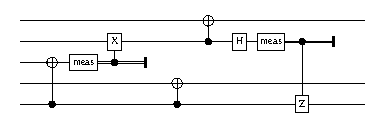
\includegraphics[scale=2]{Figures/circuits/vanillaCuts0}};
      \pic (e1) {ebit=e1/12.67mm/13mm};
      \coordinate[above left=3.6mm and -6mm of circuit.west] (leftPoint);
      \coordinate[above right=3.6mm and -6mm of circuit.east] (rightPoint);
      \pic (cut) {cut=leftPoint/rightPoint};
      \node[above left=11.5mm and -7mm of circuit.west, opacity=0.9] {\footnotesize \(A\)};
      \node[below left=4.5mm and -7mm of circuit.west, opacity=0.9] {\footnotesize \(B\)};
      \node[below left=11.5mm and -7mm of circuit.west, opacity=0.9] {\footnotesize \(C\)};
      \node[right=-3mm of circuit.north west, font=\itshape] (text) {c)};
    \end{tikzpicture}
  };
  \node[above left=-3mm and -70mm of distributed] (template) {
    \begin{tikzpicture}
      \node[inner sep=0pt] (circuit) {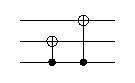
\includegraphics[scale=2]{Figures/circuits/vanillaCutsTemplate}};  
      \coordinate[above left=3.6mm and -6mm of circuit.west] (leftPoint);
      \coordinate[above right=3.6mm and -6mm of circuit.east] (rightPoint);
      \pic (cut) {cut=leftPoint/rightPoint};
      \node[above left=4.5mm and -7mm of circuit.west, opacity=0.9] {\footnotesize \(A\)};
      \node[left=-7mm of circuit.west, opacity=0.9] {\footnotesize \(B\)};
      \node[below left=4.5mm and -7mm of circuit.west, opacity=0.9] {\footnotesize \(C\)};
      \node[right=-3mm of circuit.north west, font=\itshape] (text) {a)};
    \end{tikzpicture}
  };
  \node[above right=-26.5mm and 10mm of template] (hypergraph) {
    \begin{tikzpicture}
      \coordinate (O) at (0,0);
      \coordinate (A) at (90:10mm);
      \coordinate (B) at (210:10mm);
      \coordinate (C) at (330:10mm);
      \draw (O) -- (A);
      \draw (O) -- (B);
      \draw (O) -- (C);
      \node[circle, right=-2.5mm of A, fill=white, inner sep=0pt, minimum size=5mm] {\(A\)};
      \node[circle, right=-2.5mm of B, fill=white, inner sep=0pt, minimum size=5mm] {\(B\)};
      \node[circle, right=-2.5mm of C, fill=white, inner sep=0pt, minimum size=5mm] {\(C\)};
      \coordinate[above left=5.3mm and 9mm of O] (leftPoint);
      \coordinate[above right=5.3mm and 9mm of O] (rightPoint);
      \pic (cut) {cut=leftPoint/rightPoint};
      \node[above left=0mm and 9mm of A, font=\itshape] (text) {b)};
    \end{tikzpicture}
  };
\end{tikzpicture}
\caption{The CNOTs in the circuit \textit{a)} are adjacent at their control wire. Therefore, a single hyperedge is used to represent both in \textit{b)}. The proposed cut makes only one of the CNOTs non-local, which is implemented in \textit{c)} using one ebit.}
\label{fig:vanillaCutsA}
\end{figure}

\begin{figure}
\centering
\begin{tikzpicture}
  \node (distributed) {
    \begin{tikzpicture}
      \node[inner sep=0pt] (circuit) {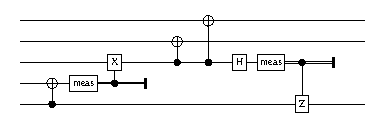
\includegraphics[scale=2]{Figures/circuits/vanillaCuts1}};
      \pic (e1) {ebit=e1/19.75mm/13mm};
      \coordinate[above left=-3.6mm and -6mm of circuit.west] (leftPoint);
      \coordinate[above right=-3.6mm and -6mm of circuit.east] (rightPoint);
      \pic (cut) {cut=leftPoint/rightPoint};
      \node[above left=11.5mm and -7mm of circuit.west, opacity=0.9] {\footnotesize \(A\)};
      \node[above left=4.5mm and -7mm of circuit.west, opacity=0.9] {\footnotesize \(B\)};
      \node[below left=11.5mm and -7mm of circuit.west, opacity=0.9] {\footnotesize \(C\)};
      \node[right=-3mm of circuit.north west, font=\itshape] (text) {c)};
    \end{tikzpicture}
  };
  \node[above left=-3mm and -70mm of distributed] (template) {
    \begin{tikzpicture}
      \node[inner sep=0pt] (circuit) {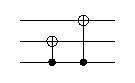
\includegraphics[scale=2]{Figures/circuits/vanillaCutsTemplate}};  
      \coordinate[below left=3.6mm and -6mm of circuit.west] (leftPoint);
      \coordinate[below right=3.6mm and -6mm of circuit.east] (rightPoint);
      \pic (cut) {cut=leftPoint/rightPoint};
      \node[above left=4.5mm and -7mm of circuit.west, opacity=0.9] {\footnotesize \(A\)};
      \node[left=-7mm of circuit.west, opacity=0.9] {\footnotesize \(B\)};
      \node[below left=4.5mm and -7mm of circuit.west, opacity=0.9] {\footnotesize \(C\)};
      \node[right=-3mm of circuit.north west, font=\itshape] (text) {a)};
    \end{tikzpicture}
  };
  \node[above right=-30mm and 10mm of template] (hypergraph) {
    \begin{tikzpicture}
      \coordinate (O) at (0,0);
      \coordinate (A) at (90:10mm);
      \coordinate (B) at (210:10mm);
      \coordinate (C) at (330:10mm);
      \draw (O) -- (A);
      \draw (O) -- (B);
      \draw (O) -- (C);
      \node[circle, right=-2.5mm of A, fill=white, inner sep=0pt, minimum size=5mm] {\(A\)};
      \node[circle, right=-2.5mm of B, fill=white, inner sep=0pt, minimum size=5mm] {\(B\)};
      \node[circle, right=-2.5mm of C, fill=white, inner sep=0pt, minimum size=5mm] {\(C\)};
      \coordinate (leftPoint) at (270:10.5mm);
      \coordinate (rightPoint) at (30:10.5mm);
      \pic (cut) {cut=leftPoint/rightPoint};
      \node[above left=0mm and 9mm of A, font=\itshape] (text) {b)};
    \end{tikzpicture}
  };
\end{tikzpicture}
\caption{Same as in Figure~\ref{fig:vanillaCutsA}, but now the cut makes both CNOTs non-local. Still, only one ebit is required, as implied by the hypergraph \textit{b)}. When CNOTs share their control wire, an ebit is required iff any of the target wires is in a different QPU than the control wire's QPU.}
\label{fig:vanillaCutsB}
\end{figure}

\begin{figure}
\hspace*{0mm}
\begin{tikzpicture}
  \node (template) {
    \begin{tikzpicture}
      \node[inner sep=0pt] (circuit) {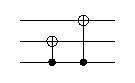
\includegraphics[scale=2]{Figures/circuits/vanillaCutsTemplate}};  
      \coordinate[below left=3.6mm and -6mm of circuit.west] (leftPoint1);
      \coordinate[below right=3.6mm and -6mm of circuit.east] (rightPoint1);
      \pic (cut1) {cut=leftPoint1/rightPoint1};
      \coordinate[above left=3.6mm and -6mm of circuit.west] (leftPoint2);
      \coordinate[above right=3.6mm and -6mm of circuit.east] (rightPoint2);
      \pic (cut2) {cut=leftPoint2/rightPoint2};
      \node[above left=4.5mm and -7mm of circuit.west, opacity=0.9] {\footnotesize \(A\)};
      \node[left=-7mm of circuit.west, opacity=0.9] {\footnotesize \(B\)};
      \node[below left=4.5mm and -7mm of circuit.west, opacity=0.9] {\footnotesize \(C\)};
      \node[right=-3mm of circuit.north west, font=\itshape] (text) {a)};
    \end{tikzpicture}
  };
  \node[above right=-28mm and 10mm of template] (hypergraph) {
    \begin{tikzpicture}
      \coordinate (O) at (0,0);
      \coordinate (A) at (90:10mm);
      \coordinate (B) at (210:10mm);
      \coordinate (C) at (330:10mm);
      \draw (O) -- (A);
      \draw (O) -- (B);
      \draw (O) -- (C);
      \node[circle, right=-2.5mm of A, fill=white, inner sep=0pt, minimum size=5mm] {\(A\)};
      \node[circle, right=-2.5mm of B, fill=white, inner sep=0pt, minimum size=5mm] {\(B\)};
      \node[circle, right=-2.5mm of C, fill=white, inner sep=0pt, minimum size=5mm] {\(C\)};
      \coordinate[above left=5.3mm and 9mm of O] (leftPoint);
      \coordinate[above right=5.3mm and 9mm of O] (rightPoint);
      \pic (cut) {cut=leftPoint/rightPoint};
      \coordinate (leftPoint2) at (270:10.5mm);
      \coordinate (rightPoint2) at (30:10.5mm);
      \pic (cut2) {cut=leftPoint2/rightPoint2};
      \coordinate (extraPoint) at (30:16mm);
      \pic (cut3) {cut=rightPoint2/extraPoint};
      \node[above left=0mm and 9mm of A, font=\itshape] (text) {b)};
    \end{tikzpicture}
  };
  \node[below right=2mm and -73mm of template] (distributed) {
    \begin{tikzpicture}[transform canvas={scale=0.65}]
      \node[inner sep=0pt] (circuit) {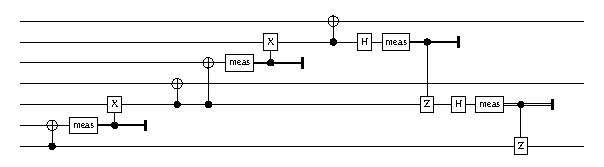
\includegraphics[scale=2]{Figures/circuits/vanillaCuts2}};
      \pic (e1) {ebit=e1/12.67mm/13mm};
      \pic (e2) {ebit=e2/33.84mm/13mm};
      \coordinate[above left=10.6mm and -6mm of circuit.west] (leftPoint);
      \coordinate[above right=10.6mm and -6mm of circuit.east] (rightPoint);
      \pic (cut) {cut=leftPoint/rightPoint};
      \coordinate[below left=10.6mm and -6mm of circuit.west] (leftPoint2);
      \coordinate[below right=10.6mm and -6mm of circuit.east] (rightPoint2);
      \pic (cut2) {cut=leftPoint2/rightPoint2};
      \node[above left=18.5mm and -7mm of circuit.west, opacity=0.9] {\footnotesize \(A\)};
      \node[left=-7mm of circuit.west, opacity=0.9] {\footnotesize \(B\)};
      \node[below left=18.5mm and -7mm of circuit.west, opacity=0.9] {\footnotesize \(C\)};
    \end{tikzpicture}
  };
  \node[right=-3mm of distributed.north west, font=\itshape] (text) {c)};
\end{tikzpicture}
\vspace*{38mm}
\caption{Same as in Figure~\ref{fig:vanillaCutsA}, but now there are two cuts, distributing the circuit across three QPUs.}
\label{fig:vanillaCutsC}
\end{figure}


\begin{figure}
\hspace*{0mm}
\begin{tikzpicture}
  \node (template) {
    \begin{tikzpicture}
      \node[inner sep=0pt] (circuit) {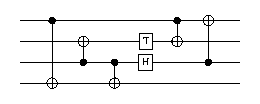
\includegraphics[scale=2]{Figures/circuits/vanillaCirc}};  
      \node[above left=8mm and -7mm of circuit.west, opacity=0.9] {\footnotesize \(A\)};
      \node[above left=1mm and -7mm of circuit.west, opacity=0.9] {\footnotesize \(B\)};
      \node[below left=1mm and -7mm of circuit.west, opacity=0.9] {\footnotesize \(C\)};
      \node[below left=8mm and -7mm of circuit.west, opacity=0.9] {\footnotesize \(D\)};
      \node[right=-3mm of circuit.north west, font=\itshape] (text) {a)};
    \end{tikzpicture}
  };
  \node[above right=-35.5mm and 6mm of template] (hypergraph) {
    \begin{tikzpicture}
      \coordinate (O) at (0,0);
      \coordinate (B) at (45:13mm);
      \coordinate (A) at (135:13mm);
      \coordinate (C) at (225:13mm);
      \coordinate (D) at (315:13mm);
      \coordinate (auxB) at (45:4.5mm);
      \coordinate (auxD) at (315:4.5mm);
      \draw (A) -- (C);
      \draw (A) -- (auxB);
      \draw (B) -- (auxB);
      \draw (D) -- (auxB);
      \draw (C) -- (auxD);
      \draw (B) -- (auxD);
      \draw (D) -- (auxD);
      \node[circle, right=-2.5mm of A, fill=white, inner sep=0pt, minimum size=5mm] {\(A\)};
      \node[circle, right=-2.5mm of B, fill=white, inner sep=0pt, minimum size=5mm] {\(B\)};
      \node[circle, right=-2.5mm of C, fill=white, inner sep=0pt, minimum size=5mm] {\(C\)};
      \node[circle, right=-2.5mm of D, fill=white, inner sep=0pt, minimum size=5mm] {\(D\)};
      \coordinate[above left=9mm and 1mm of O] (leftPoint);
      \coordinate[below left=9mm and 1mm of O] (rightPoint);
      \pic (cut) {cut=leftPoint/rightPoint};
      \node[above left=5mm and 9mm of A, font=\itshape] (text) {b)};
    \end{tikzpicture}
  };
  \node[below right=4mm and -92mm of template] (distributed) {
    \begin{tikzpicture}[transform canvas={scale=0.58}]
      \node[inner sep=0pt] (circuit) {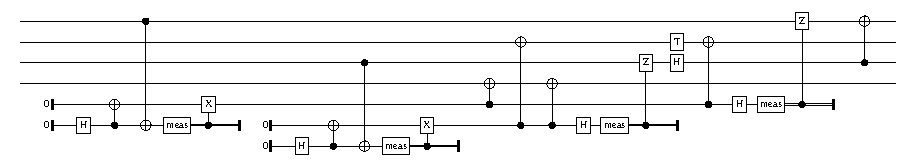
\includegraphics[scale=2]{Figures/circuits/vanillaDistrib}};
      \pic (e2) {ebitLong=e2/19.76mm/15.5mm};
      \pic (e1) {ebitLessClear=e1/26.8mm/16mm};
      \coordinate[left=-4mm of circuit.west] (leftPoint);
      \coordinate[right=-4mm of circuit.east] (rightPoint);
      \pic (cut) {cut=leftPoint/rightPoint};
      \node[above left=22mm and -7mm of circuit.west, opacity=0.9] {\(B\)};
      \node[above left=15mm and -7mm of circuit.west, opacity=0.9] {\(D\)};
      \node[below left=15mm and -7mm of circuit.west, opacity=0.9] {\(A\)};
      \node[below left=22mm and -7mm of circuit.west, opacity=0.9] {\(C\)};
    \end{tikzpicture}
  };
  \node[right=-1mm of distributed.north west, font=\itshape] (text) {c)};
\end{tikzpicture}
\vspace*{38mm}
\caption{The circuit is distributed using only \(2\) ebits. The other two possible distributions: \(\{\{A,B\},\{C,D\}\}\) and \(\{\{A,D\},\{B,C\}\}\) both require \(3\) ebits to be implemented. The wires in the distributed version of the circuit have been rearranged, so it is possible to visualise in a planar diagram that no quantum information crosses the boundary.}
\label{fig:vanillaExample}
\end{figure}


A simple circuit, its optimally partitioned hypergraph and the resulting distributed circuit are shown in Figure~\ref{fig:vanillaExample}. The obtained distribution is the most efficient one, in the sense described in the beginning of this section. Each of the QPUs can be set to implement its own local circuit, distilling ebits and using them along classical communication whenever indicated.


\subsection{Bringing CNOT gates together}
\label{pullCNOTs}

In \S\ref{NonLocalGates} we have shown that any 1-qubit gate in the Clifford+T set acting on the control wire of a CNOT gate, with the exception of the H gate, can commute with the CNOT up to some byproduct. Here we use this fact, applying some pre-processing on the input circuit that brings together nearby CNOT gates, allowing us to implement more non-local CNOT gates using a single ebit. Figure~\ref{fig:pulledCNOTexample} gives an example of how these transformations -- listed in Figure~\ref{fig:pullRules} -- can lead to a more efficient distribution of the circuit.

\begin{figure}
\centering
\begin{tikzpicture}
  \node (circ) {
    \begin{tikzpicture}
      \node[inner sep=0pt] (circuit) {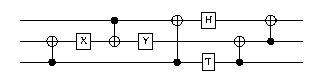
\includegraphics[scale=2, trim={2.5mm 0 2.5mm 0}, clip]{Figures/circuits/pullCirc}};  
      \node[left=-7mm of circuit.west, rectangle,fill=white,minimum height=22mm, minimum width=8mm] {};
      \node[right=-7mm of circuit.east, rectangle,fill=white,minimum height=22mm, minimum width=8mm] {};
      \node[above left=4.5mm and -7mm of circuit.west, opacity=0.9] {\footnotesize \(A\)};
      \node[left=-7mm of circuit.west, opacity=0.9] {\footnotesize \(B\)};
      \node[below left=4.5mm and -7mm of circuit.west, opacity=0.9] {\footnotesize \(C\)};
      \node[right=-3mm of circuit.north west, font=\itshape] (text) {a)};
    \end{tikzpicture}
  };
  \node[below=5mm of circ] (pulled) {
    \begin{tikzpicture}
      \node[inner sep=0pt] (circuit) {\includegraphics[scale=2, trim={2.5mm 0 2.5mm 0}, clip]{Figures/circuits/pullPulled}};  
      \node[left=-7mm of circuit.west, rectangle,fill=white,minimum height=22mm, minimum width=8mm] {};
      \node[right=-7mm of circuit.east, rectangle,fill=white,minimum height=22mm, minimum width=8mm] {};
      \node[above left=4.5mm and -7mm of circuit.west, opacity=0.9] {\footnotesize \(A\)};
      \node[left=-7mm of circuit.west, opacity=0.9] {\footnotesize \(B\)};
      \node[below left=4.5mm and -7mm of circuit.west, opacity=0.9] {\footnotesize \(C\)};
      \node[right=-3mm of circuit.north west, font=\itshape] (text) {c)};
    \end{tikzpicture}
  };
  \node[above right=-32.5mm and -2mm of circ] (hypergraph) {
    \begin{tikzpicture}
      \coordinate (O) at (0,0);
      \coordinate (A) at (90:12mm);
      \coordinate (B) at (210:12mm);
      \coordinate (C) at (330:12mm);
      \draw (O) -- (A);
      \draw (O) -- (B);
      \draw (O) -- (C);
      \draw (A) edge[out=210,in=90,looseness=1] (B); 
      \draw (A) -- (B);
      \draw (B) -- (C);
      \node[circle, right=-2.5mm of A, fill=white, inner sep=0pt, minimum size=5mm] {\(A\)};
      \node[circle, right=-2.5mm of B, fill=white, inner sep=0pt, minimum size=5mm] {\(B\)};
      \node[circle, right=-2.5mm of C, fill=white, inner sep=0pt, minimum size=5mm] {\(C\)};
      \coordinate (leftPoint) at (270:11.5mm);
      \coordinate (rightPoint) at (30:11.5mm);
      \pic (cut) {cut=leftPoint/rightPoint};
      \node[above left=0mm and 13mm of A, font=\itshape] (text) {b)};
    \end{tikzpicture}
  };
  \node[above right=-32.5mm and -2mm of pulled] (hypergraph2) {
    \begin{tikzpicture}
      \coordinate (O) at (0,0);
      \coordinate (A) at (90:12mm);
      \coordinate (B) at (210:12mm);
      \coordinate (C) at (330:12mm);
      \draw (O) -- (A);
      \draw (O) -- (B);
      \draw (O) -- (C);
      \draw (A) edge[out=210,in=90,looseness=1] (B); 
      \draw (A) -- (B);
      \node[circle, right=-2.5mm of A, fill=white, inner sep=0pt, minimum size=5mm] {\(A\)};
      \node[circle, right=-2.5mm of B, fill=white, inner sep=0pt, minimum size=5mm] {\(B\)};
      \node[circle, right=-2.5mm of C, fill=white, inner sep=0pt, minimum size=5mm] {\(C\)};
      \coordinate (leftPoint) at (270:11.5mm);
      \coordinate (rightPoint) at (30:11.5mm);
      \pic (cut) {cut=leftPoint/rightPoint};
      \node[above left=0mm and 13mm of A, font=\itshape] (text) {d)};
    \end{tikzpicture}
  };
\end{tikzpicture}
\vspace*{5mm}
\caption{Example where an ebit can be saved by sliding CNOTs closer together. This figure shows the original circuit \textit{a)}, its optimally partitioned hypergraph \textit{b)}, the pre-processed circuit \textit{c)}, and its optimally partitioned hypergraph \textit{d)}, which has one less cut hyperedge.}
\label{fig:pulledCNOTexample}
\end{figure}

The pre-processing procedure is fairly straight-forward: Exploring the circuit from left to right, whever a CNOT gate is found, use the transformations listed in Figure~\ref{fig:pullRules} to move it as early in the circuit as possible. The procedure introduces some additional \(X\) gates. Fortunately, \(X\) is its own inverse (i.e.\ \(XX = I\)) and every 1-qubit gate in Clifford+T can be interchanged with \(X\) in a simple way (as shown in Figure~\ref{fig:props}). Hence, we should not expect a significant increase in the depth of the circuit, as most byproduct gates will cancel each other out.

So far we have been talking about standard 1-qubit gates, but in practical circuits we are likely to find 1-qubit gates that are \textit{classically-controlled}, meaning that a classical signal (a bit, either \(0\) or \(1\)) decides whether the gate is applied or not. These are no issue for the distribution of the circuit, as this classical control may only require classical communication between QPUs. Concerning the pre-processing we just described, classically-controlled 1-qubit gates can commute with CNOT under the exact same circumstances as their uncontrolled version. The only difference is that, whenever a byproduct gate is created, we must make sure it is controlled by the same classical signal that controlled the original gate, as shown in Figure~\ref{fig:classicalControl}.

\begin{figure}
\centering
\begin{tikzpicture}
  \node {
    \begin{tikzpicture}
      \node[inner sep=0pt] (circuit) at (0,0) {\includegraphics[scale=2]{Figures/circuits/classicalControl}};
      \node[right=0mm of circuit.north west, font=\itshape] (text) {a)};
    \end{tikzpicture}
    \hspace{8mm}
    \begin{tikzpicture}
      \node[inner sep=0pt] (circuit) at (0,0) {\includegraphics[scale=2]{Figures/circuits/classicalControl2}};
      \node[right=0mm of circuit.north west, font=\itshape] (text) {b)};
    \end{tikzpicture}
  };
\end{tikzpicture}
\caption{Pushing a classically controlled gate through a CNOT. The same rule as in Figure~\ref{fig:pullRules} is applied, while making sure any new gate is also controlled. Here, only the case for \(X\) gate is shown, but this works for any of the transformations in Figure~\ref{fig:pullRules}.}
\label{fig:classicalControl}
\end{figure}

The same procedure can be used to commute 1-qubit gates across the target wire of the CNOT gates, although in this case, apart from \(H\), \(S\) and \(T\) gates can not commute either. This additional pre-processing would have no effect at all on the vanilla version of the algorithm, but it will be beneficial after we apply our next extension, which requires CNOT gates to be adjacent on the target wire.


\subsection{Using the remote-target method}
\label{BothEnds}

In \S\ref{NonLocalGates} we showed that the trick for implementing multiple CNOT gates using a single ebit also works if they share a common target wire (instead of the control wire). This makes our optimisation problem more intricate: Now, when the CNOTs are to be implemented non-locally, we can choose to implement them using the remote-control or remote-target method. For explanation purposes, we will use two different kinds of hyperedges in this subsection's figures, depending on whether their CNOTs are controlled by the same wire, or act on the same target (thicker line). 

\begin{figure}
\centering
\begin{tikzpicture}
  \node (circ) {
    \begin{tikzpicture}
      \node[inner sep=0pt] (circuit) {\includegraphics[scale=2]{Figures/circuits/bothEndsSimple}};  
      \node[above left=4.5mm and -7mm of circuit.west, opacity=0.9] {\footnotesize \(A\)};
      \node[left=-7mm of circuit.west, opacity=0.9] {\footnotesize \(B\)};
      \node[below left=4.5mm and -7mm of circuit.west, opacity=0.9] {\footnotesize \(C\)};
      \node[above right=0.8mm and 12.8mm of circuit.west, opacity=0.9] {\footnotesize \(\gamma\)};
      \node[below right=0.8mm and 23.6mm of circuit.west, opacity=0.9] {\footnotesize \(\beta\)};
      \node[below right=0.8mm and 34.4mm of circuit.west, opacity=0.9] {\footnotesize \(\alpha\)};
      \node[right=-3mm of circuit.north west, font=\itshape] (text) {a)};
    \end{tikzpicture}
  };
  \node[above right=-27mm and 5mm of circ] (controlHyp) {
    \begin{tikzpicture}
      \coordinate (O) at (0,0);
      \coordinate (A) at (90:10mm);
      \coordinate (B) at (210:10mm);
      \coordinate (C) at (330:10mm);
      \draw (O) -- (A);
      \draw (O) -- (B);
      \draw (O) -- (C);
      \draw (B) -- (C);
      \node[circle, right=-2.5mm of A, fill=white, inner sep=0pt, minimum size=5mm] {\(A\)};
      \node[circle, right=-2.5mm of B, fill=white, inner sep=0pt, minimum size=5mm] {\(B\)};
      \node[circle, right=-2.5mm of C, fill=white, inner sep=0pt, minimum size=5mm] {\(C\)};
      \node[above left=0mm and 13mm of A, font=\itshape] (text) {b)};
    \end{tikzpicture}
  };
  \node[right=-27mm and 15mm of circ] (targetHyp) {
    \begin{tikzpicture}
      \coordinate (O) at (0,0);
      \coordinate (A) at (90:10mm);
      \coordinate (B) at (210:10mm);
      \coordinate (C) at (330:10mm);
      \draw[ultra thick] (O) -- (A);
      \draw[ultra thick] (O) -- (B);
      \draw[ultra thick] (O) -- (C);
      \draw[ultra thick] (A) -- (B);
      \node[circle, right=-2.5mm of A, fill=white, inner sep=0pt, minimum size=5mm] {\(A\)};
      \node[circle, right=-2.5mm of B, fill=white, inner sep=0pt, minimum size=5mm] {\(B\)};
      \node[circle, right=-2.5mm of C, fill=white, inner sep=0pt, minimum size=5mm] {\(C\)};
      \node[above left=0mm and 13mm of A, font=\itshape] (text) {c)};
    \end{tikzpicture}
  };
  \node[below right=0mm and 0mm of circ] (bothHyp) {
    \begin{tikzpicture}
      \coordinate (O) at (0,0);
      \coordinate (auxC) at (4mm,3mm);
      \coordinate (auxT) at (-4mm,3mm);
      \coordinate (A) at (90:20mm);
      \coordinate (B) at (210:20mm);
      \coordinate (C) at (330:20mm);
      \draw[ultra thick] (auxT) -- (A);
      \draw[ultra thick] (auxT) -- (B);
      \draw[ultra thick] (auxT) -- (C);
      \draw[ultra thick] (A) -- (B);
      \draw (auxC) -- (A);
      \draw (auxC) -- (B);
      \draw (auxC) -- (C);
      \draw (B) -- (C);
      \node[circle, right=-2.5mm of A, fill=white, inner sep=0pt, minimum size=5mm] {\(A\)};
      \node[circle, right=-2.5mm of B, fill=white, inner sep=0pt, minimum size=5mm] {\(B\)};
      \node[circle, right=-2.5mm of C, fill=white, inner sep=0pt, minimum size=5mm] {\(C\)};
      \node[above left=0mm and 13mm of A, font=\itshape] (text) {c)};
    \end{tikzpicture}
  };
  \node[right=5mm of bothHyp] (hypergraph) {
    \begin{tikzpicture}
      \coordinate (O) at (0,0);
      \coordinate (auxA) at (90:9mm);
      \coordinate (auxC) at (330:9mm);
      \coordinate (A) at (90:18mm);
      \coordinate (B) at (210:18mm);
      \coordinate (C) at (330:18mm);
      \coordinate (a) at (270:9mm);
      \coordinate (b) at (30:9mm);
      \coordinate (c) at (150:9mm);
      \draw (auxA) -- (A);
      \draw (auxA) -- (b);
      \draw (auxA) -- (c);
      \draw[ultra thick] (auxC) -- (C);
      \draw[ultra thick] (auxC) -- (b);
      \draw[ultra thick] (auxC) -- (a);
      \draw (B) -- (a);
      \draw[ultra thick] (B) -- (c);
      \node[circle, right=-2.5mm of A, fill=white, inner sep=0pt, minimum size=5mm] {\(A\)};
      \node[circle, right=-2.5mm of B, fill=white, inner sep=0pt, minimum size=5mm] {\(B\)};
      \node[circle, right=-2.5mm of C, fill=white, inner sep=0pt, minimum size=5mm] {\(C\)};
      \node[circle, right=-2.5mm of a, fill=white, inner sep=0pt, minimum size=5mm] {\(\alpha\)};
      \node[circle, right=-2.5mm of b, fill=white, inner sep=0pt, minimum size=5mm] {\(\beta\)};
      \node[circle, right=-2.5mm of c, fill=white, inner sep=0pt, minimum size=5mm] {\(\gamma\)};
      \node[above left=0mm and 13mm of A, font=\itshape] (text) {e)};
    \end{tikzpicture}
  };
\end{tikzpicture}
\vspace*{5mm}
\caption{}
\label{fig:BothEndsChallenge}
\end{figure}

\textbf{TODO}: If the partition is \(\{\{A\},\{B,C\}\}\), then \(\alpha\) is a local CNOT, while \(\beta\) and \(\gamma\) are implemented using the common-control method. We know the common-control method must be used because the hyperedge cut is of the control type or, equivalently, because both \(\beta\) and \(\gamma\) vertices are assigned to the same block as their targets \(C\) and \(B\). Different line format for the hyperedges whether control or target.

\textbf{TODO}: Show cut that is best for common-target

\textbf{TODO}: Figure of hypergraphs from prev Fig; with control hyps, target hyps, naively. The dashed lines represent two hypothetical ways of partitioning the hypergraph. Different line format for the hyperedges whether control or target (fig:BothEndsChallenge)

Figure~\ref{fig:BothEndsChallenge}\textit{a)} shows a simple circuit where a CNOT \(\beta\) shares its target wire \(C\) with another CNOT \(\alpha\). The remote-target method would allow to implement these two non-locally, using a single ebit. We represent this fact in hypergraph \textit{c)}, as the three-vertex hyperedge. Gate \(\gamma\) shares its target with no other gate, so it is represented with an edge \((A,B)\). Hypergraph \textit{b)} is the one built by Algorithm~\ref{code:BuildHypVanilla}, and considers all non-local CNOTs are implemented as remote-control, so it is now gate \(\alpha\) the isolated edge \((B,C)\). If we were to partition the circuit as shown in the figure, hypergraph \textit{b)} would suggest that two qubits are required, when actually only one is enough, as shown by hypergraph \textit{c)}. But, if the partition is \(\{\{A\},\{B,C\}\}\) instead, hypergraph \textit{c)} would be the one overestimating the number of ebits needed. Hence, both hypergraphs \textit{b)} and \textit{c)} are biased. 

If we want to guarantee that the most efficient circuit distribution can always be found by a graph partitioner, we must find an alternative hypergraph representation of the circuit. Notice that it is not an option to simply find the optimal partition for both hypergraphs \textit{b)} and \textit{c)} and choose the one with least cuts: The best circuit distribution is unlikely to have all its CNOTs implemented in the same way. Therefore, our hypergraph representation must have the following characteristics:
\begin{enumerate}
  \item Both options of how to implement each CNOT are represented.
  \item A partition of the hypergraph must determine, for each non-local CNOT, which method should be used to implement it.
  \item The \(\lambda-1\) metric of a partition should accurately determine how many ebits are required to implement the circuit distribution it describes.
\end{enumerate}

\begin{algorithm}[caption={Builds the hypergraph of a given circuit, without choosing whether CNOT gates are implemented through common control or common target. This algorithm runs in time \(O(g)\), where \(g\) is the number of gates in the input circuit.}, label={code:buildHypBothEnds}]
input: circuit
output: (V,H)
begin
  V $\gets$ $\varnothing$
  H $\gets$ $\varnothing$
  hedge $\gets$ $\varnothing$
  foreach wire in circuit do
    V $\gets$ V $\cup$ {wire}
    H $\gets$ H $+$ {hedge}
    hedge $\gets$ {wire}
    hType $\gets$ $unknown$
    foreach gate in wire do
      V $\gets$ V $\cup$ {$labelOf$(gate)}
      if gate == CNOT then
        if $controlOf$(gate) == wire then
          if hType == $target$ then
            H $\gets$ H $+$ {hedge}
            hedge $\gets$ {wire}
          hType $\gets$ $control$
        if $targetOf$(gate) == wire then
          if hType == $control$ then
            H $\gets$ H $+$ {hedge}
            hedge $\gets$ {wire}  
          hType $\gets$ $target$
        hedge $\gets$ hedge $\cup$ {$labelOf$(gate)}
      else
        H $\gets$ H $+$ {hedge}
        hType $\gets$ $unknown$
        hedge $\gets$ {wire}
end
\end{algorithm}

\begin{figure}
\centering
\begin{tikzpicture}
  \node (circ) {
    \begin{tikzpicture}
      \node[inner sep=0pt] (circuit) {\includegraphics[scale=2]{Figures/circuits/bothEndsSimple}};  
      \node[above left=4.5mm and -7mm of circuit.west, opacity=0.9] {\footnotesize \(A\)};
      \node[left=-7mm of circuit.west, opacity=0.9] {\footnotesize \(B\)};
      \node[below left=4.5mm and -7mm of circuit.west, opacity=0.9] {\footnotesize \(C\)};
      \node[above right=0.8mm and 12.8mm of circuit.west, opacity=0.9] {\footnotesize \(\gamma\)};
      \node[below right=0.8mm and 23.6mm of circuit.west, opacity=0.9] {\footnotesize \(\beta\)};
      \node[below right=0.8mm and 34.4mm of circuit.west, opacity=0.9] {\footnotesize \(\alpha\)};
      \node[right=-3mm of circuit.north west, font=\itshape] (text) {Input:};
    \end{tikzpicture}
  };
  \node[right=3mm of circ] (step1) {
    \begin{tikzpicture}
      \coordinate (O) at (0,0);
      \coordinate (auxA) at (90:9mm);
      \coordinate (auxC) at (330:9mm);
      \coordinate (A) at (90:18mm);
      \coordinate (B) at (210:18mm);
      \coordinate (C) at (330:18mm);
      \coordinate (a) at (270:9mm);
      \coordinate (b) at (30:9mm);
      \coordinate (c) at (150:9mm);
      \draw (auxA) -- (A);
      %\draw (auxA) -- (b);
      \draw (auxA) -- (c);
      %\draw[ultra thick] (auxC) -- (C);
      %\draw[ultra thick] (auxC) -- (b);
      %\draw[ultra thick] (auxC) -- (a);
      %\draw (B) -- (a);
      %\draw[ultra thick] (B) -- (c);
      \node[circle, right=-2.5mm of A, fill=white, inner sep=0pt, minimum size=5mm] {\(A\)};
      %\node[circle, right=-2.5mm of B, fill=white, inner sep=0pt, minimum size=5mm] {\(B\)};
      %\node[circle, right=-2.5mm of C, fill=white, inner sep=0pt, minimum size=5mm] {\(C\)};
      %\node[circle, right=-2.5mm of a, fill=white, inner sep=0pt, minimum size=5mm] {\(\alpha\)};
      %\node[circle, right=-2.5mm of b, fill=white, inner sep=0pt, minimum size=5mm] {\(\beta\)};
      \node[circle, right=-2.5mm of c, fill=white, inner sep=0pt, minimum size=5mm] {\(\gamma\)};
      \node[above left=0mm and 13mm of A, font=\itshape] (text) {1)};
    \end{tikzpicture}
  };
  \node[right=16.5mm of step1] (step2) {
    \begin{tikzpicture}
      \coordinate (O) at (0,0);
      \coordinate (auxA) at (90:9mm);
      \coordinate (auxC) at (330:9mm);
      \coordinate (A) at (90:18mm);
      \coordinate (B) at (210:18mm);
      \coordinate (C) at (330:18mm);
      \coordinate (a) at (270:9mm);
      \coordinate (b) at (30:9mm);
      \coordinate (c) at (150:9mm);
      \draw (auxA) -- (A);
      \draw (auxA) -- (b);
      \draw (auxA) -- (c);
      %\draw[ultra thick] (auxC) -- (C);
      %\draw[ultra thick] (auxC) -- (b);
      %\draw[ultra thick] (auxC) -- (a);
      %\draw (B) -- (a);
      %\draw[ultra thick] (B) -- (c);
      \node[circle, right=-2.5mm of A, fill=white, inner sep=0pt, minimum size=5mm] {\(A\)};
      %\node[circle, right=-2.5mm of B, fill=white, inner sep=0pt, minimum size=5mm] {\(B\)};
      %\node[circle, right=-2.5mm of C, fill=white, inner sep=0pt, minimum size=5mm] {\(C\)};
      %\node[circle, right=-2.5mm of a, fill=white, inner sep=0pt, minimum size=5mm] {\(\alpha\)};
      \node[circle, right=-2.5mm of b, fill=white, inner sep=0pt, minimum size=5mm] {\(\beta\)};
      \node[circle, right=-2.5mm of c, fill=white, inner sep=0pt, minimum size=5mm] {\(\gamma\)};
      \node[above left=0mm and 13mm of A, font=\itshape] (text) {2)};
    \end{tikzpicture}
  };
  \node[below left=5mm and -30mm of circ] (step3) {
    \begin{tikzpicture}
      \coordinate (O) at (0,0);
      \coordinate (auxA) at (90:9mm);
      \coordinate (auxC) at (330:9mm);
      \coordinate (A) at (90:18mm);
      \coordinate (B) at (210:18mm);
      \coordinate (C) at (330:18mm);
      \coordinate (a) at (270:9mm);
      \coordinate (b) at (30:9mm);
      \coordinate (c) at (150:9mm);
      \draw (auxA) -- (A);
      \draw (auxA) -- (b);
      \draw (auxA) -- (c);
      %\draw[ultra thick] (auxC) -- (C);
      %\draw[ultra thick] (auxC) -- (b);
      %\draw[ultra thick] (auxC) -- (a);
      %\draw (B) -- (a);
      \draw[ultra thick] (B) -- (c);
      \node[circle, right=-2.5mm of A, fill=white, inner sep=0pt, minimum size=5mm] {\(A\)};
      \node[circle, right=-2.5mm of B, fill=white, inner sep=0pt, minimum size=5mm] {\(B\)};
      %\node[circle, right=-2.5mm of C, fill=white, inner sep=0pt, minimum size=5mm] {\(C\)};
      %\node[circle, right=-2.5mm of a, fill=white, inner sep=0pt, minimum size=5mm] {\(\alpha\)};
      \node[circle, right=-2.5mm of b, fill=white, inner sep=0pt, minimum size=5mm] {\(\beta\)};
      \node[circle, right=-2.5mm of c, fill=white, inner sep=0pt, minimum size=5mm] {\(\gamma\)};
      \node[above left=0mm and 13mm of A, font=\itshape] (text) {3)};
    \end{tikzpicture}
  };
  \node[right=20mm of step3] (step4) {
    \begin{tikzpicture}
      \coordinate (O) at (0,0);
      \coordinate (auxA) at (90:9mm);
      \coordinate (auxC) at (330:9mm);
      \coordinate (A) at (90:18mm);
      \coordinate (B) at (210:18mm);
      \coordinate (C) at (330:18mm);
      \coordinate (a) at (270:9mm);
      \coordinate (b) at (30:9mm);
      \coordinate (c) at (150:9mm);
      \draw (auxA) -- (A);
      \draw (auxA) -- (b);
      \draw (auxA) -- (c);
      %\draw[ultra thick] (auxC) -- (C);
      %\draw[ultra thick] (auxC) -- (b);
      %\draw[ultra thick] (auxC) -- (a);
      \draw (B) -- (a);
      \draw[ultra thick] (B) -- (c);
      \node[circle, right=-2.5mm of A, fill=white, inner sep=0pt, minimum size=5mm] {\(A\)};
      \node[circle, right=-2.5mm of B, fill=white, inner sep=0pt, minimum size=5mm] {\(B\)};
      %\node[circle, right=-2.5mm of C, fill=white, inner sep=0pt, minimum size=5mm] {\(C\)};
      \node[circle, right=-2.5mm of a, fill=white, inner sep=0pt, minimum size=5mm] {\(\alpha\)};
      \node[circle, right=-2.5mm of b, fill=white, inner sep=0pt, minimum size=5mm] {\(\beta\)};
      \node[circle, right=-2.5mm of c, fill=white, inner sep=0pt, minimum size=5mm] {\(\gamma\)};
      \node[above left=0mm and 13mm of A, font=\itshape] (text) {4)};
    \end{tikzpicture}
  };
  \node[right=20mm of step4] (final) {
    \begin{tikzpicture}
      \coordinate (O) at (0,0);
      \coordinate (auxA) at (90:9mm);
      \coordinate (auxC) at (330:9mm);
      \coordinate (A) at (90:18mm);
      \coordinate (B) at (210:18mm);
      \coordinate (C) at (330:18mm);
      \coordinate (a) at (270:9mm);
      \coordinate (b) at (30:9mm);
      \coordinate (c) at (150:9mm);
      \draw (auxA) -- (A);
      \draw (auxA) -- (b);
      \draw (auxA) -- (c);
      \draw[ultra thick] (auxC) -- (C);
      \draw[ultra thick] (auxC) -- (b);
      \draw[ultra thick] (auxC) -- (a);
      \draw (B) -- (a);
      \draw[ultra thick] (B) -- (c);
      \node[circle, right=-2.5mm of A, fill=white, inner sep=0pt, minimum size=5mm] {\(A\)};
      \node[circle, right=-2.5mm of B, fill=white, inner sep=0pt, minimum size=5mm] {\(B\)};
      \node[circle, right=-2.5mm of C, fill=white, inner sep=0pt, minimum size=5mm] {\(C\)};
      \node[circle, right=-2.5mm of a, fill=white, inner sep=0pt, minimum size=5mm] {\(\alpha\)};
      \node[circle, right=-2.5mm of b, fill=white, inner sep=0pt, minimum size=5mm] {\(\beta\)};
      \node[circle, right=-2.5mm of c, fill=white, inner sep=0pt, minimum size=5mm] {\(\gamma\)};
      \node[above left=0mm and 13mm of A, font=\itshape] (text) {5)};
    \end{tikzpicture}
  };
\end{tikzpicture}
\vspace*{0mm}
\caption{Step by step execution of Algorithm~\ref{code:buildHypBothEnds}.}
\label{fig:BothEndsProcess}
\end{figure}

We propose our new hypergraph representation to be as \textit{d)} from Figure~\ref{fig:BothEndsChallenge}. Algorithm~\ref{code:BuildHypBothEnds} builds such a hypergraph for any given circuit, and Figure~\ref{fig:BothEndsProcess} shows how the hypergraph is built step by step for our running example. These hypergraphs satisfy the three requirements defined above: First, we include all of the control-hyperedges and target-hyperedges. For the second requirement, we give additional structure to the hypergraph, adding vertices that represent CNOT gates; how a CNOT is implemented will be determined by the block its CNOT-vertex is assigned to. The third requirement is the most subtle one. Intuitively, we satisfy it by, imposing that each CNOT-vertex participates in only two hyperedges; one connecting it to its control wire-vertex, the other to its target. A more detailed account of how this third requirement holds is given in the proof of Theorem~\ref{thm:bothEnds}. Corollary~\ref{col:bothEnds} confirms that the optimal partition of our hypergraph determines the most efficient circuit distribution.


\begin{theorem}
 Given any circuit \(\mathcal{C}\), and its hypergraph \(\mathcal{H}\) generated by Algorithm~\ref{code:buildHypBothEnds}, there is a bijection between partitions of \(\mathcal{H}\) with \(\lambda_c\) cuts and distributions of \(\mathcal{C}\) using \(\lambda_e\) ebits.
 \label{thm:bothEnds}
\end{theorem}
\begin{proof}
We define the same trivial configuration in Theorem~\ref{thm:vanilla}. In the case of \S\ref{Vanilla}, the CNOT operation itself was always applied in the same QPU as its target, regardless of the CNOT being local or not (see Figure~\ref{fig:nonlocalCNOTs}). Thus, the primitive from Theorem~\ref{thm:vanilla} for moving a wire-vertex \(x\) around is defined here with the extra constraint that all CNOT-vertices connected by a target-hyperedge to \(x\) must move with it to the same block/QPU \(x\) does. 

In order to reach any hypergraph partition we need to add a primitive that allows us to move a CNOT-vertex \(x\) independently from its wire-vertices. Conversely, in order to reach any arbitrary circuit distribution, we need to be able to change the QPU where a CNOT gate \(x\) is implemented. This pair of primitives is defined to correspond one-to-one to each other. Let's consider the four distinct cases of how \(x\) may be allocated regarding its neighbouring wire-vertices acting as CNOT \(x\)'s control \(c_x\) and target \(t_x\):
\begin{itemize}
  \item \textit{Local}: The three vertices \(x\), \(c_x\) and \(t_x\) are in the same block \(i\). In this case, \(x\)'s allocation contributes to neither a cut on its control-hyperedge nor a cut on its target-hyperedge. The CNOT gate is implemented locally in QPU \(i\), so no ebit is required to implement it.
  \item \textit{Remote control}: Both \(x\) and \(t_x\) are in a block \(i\), while \(c_x\) is in a different block \(j\). In this case, \(x\)'s allocation contributes only to a cut on its control-hyperedge. An ebit is required to implement the CNOT, which may be also used to implement other CNOTs in QPU \(i\) that are also controlled by \(c_x\). This is the case from Figure~\ref{fig:nonlocalCNOTs}, and the only one available for the implementation of non-local CNOTs in the vanilla algorithm.
  \item \textit{Remote target}: Both \(x\) and \(c_x\) are in a block \(i\), while \(t_x\) is in a different block \(j\). In this case, \(x\)'s allocation contributes only to a cut on its target-hyperedge. Again, an ebit is required to implement the CNOT, although in this case other CNOTs in QPU \(i\) with common \(t_x\) target may share that ebit.
  \item \textit{External}: The three vertices are in separated blocks, with \(x\) in some block \(i\). An example of this situation is shown in Figure~\ref{fig:farCNOT}. In this case, \(x\)'s allocation contributes to both a cut on its control-hyperedge and on its target-hyperedge. In this case, two ebits are required; the one used to access \(c_x\) may be shared with other CNOT gates in \(i\) that have that wire as common control, while the ebit used to access \(t_x\) may be shared with CNOTs in \(i\) that have that target in common.
\end{itemize} 

The proof by induction discussed in Theorem~\ref{thm:vanilla} holds here if we manage to show that any application of this CNOT-vertex allocation primitive still preserves \(\lambda_c = \lambda_e\). Changing the allocation of a CNOT-vertex \(x\) may change its situation among the four cases above. As detailed there, in each case \(x\)'s allocation contributes to the same amount of cuts as ebits the CNOT \(x\) requires. Hence, changing the allocation of \(x\) always preserves \(\lambda_c = \lambda_e\).

\end{proof}

\begin{figure}[h]
\hspace*{-8mm}
\begin{tikzpicture}
  \node (circ) {
    \begin{tikzpicture}
      \node[inner sep=0pt] (circuit) {\includegraphics[scale=2]{Figures/circuits/bothEndsSimple}};  
      \node[above left=4.5mm and -7mm of circuit.west, opacity=0.9] {\footnotesize \(A\)};
      \node[left=-7mm of circuit.west, opacity=0.9] {\footnotesize \(B\)};
      \node[below left=4.5mm and -7mm of circuit.west, opacity=0.9] {\footnotesize \(C\)};
      \node[above right=0.8mm and 12.8mm of circuit.west, opacity=0.9] {\footnotesize \(\gamma\)};
      \node[below right=0.8mm and 23.6mm of circuit.west, opacity=0.9] {\footnotesize \(\beta\)};
      \node[below right=0.8mm and 34.4mm of circuit.west, opacity=0.9] {\footnotesize \(\alpha\)};
      \node[right=-3mm of circuit.north west, font=\itshape] (text) {a)};
    \end{tikzpicture}
  };
  \node[below right=-40mm and 20mm of circ] (hypergraph) {
    \begin{tikzpicture}
      \coordinate (O) at (0,0);
      \coordinate (auxA) at (90:9mm);
      \coordinate (auxC) at (330:9mm);
      \coordinate (A) at (90:18mm);
      \coordinate (B) at (210:18mm);
      \coordinate (C) at (330:18mm);
      \coordinate (a) at (270:9mm);
      \coordinate (b) at (30:9mm);
      \coordinate (c) at (150:9mm);
      \draw (auxA) -- (A);
      \draw (auxA) -- (b);
      \draw (auxA) -- (c);
      \draw[ultra thick] (auxC) -- (C);
      \draw[ultra thick] (auxC) -- (b);
      \draw[ultra thick] (auxC) -- (a);
      \draw (B) -- (a);
      \draw[ultra thick] (B) -- (c);
      \node[circle, right=-2.5mm of A, fill=white, inner sep=0pt, minimum size=5mm] {\(A\)};
      \node[circle, right=-2.5mm of B, fill=white, inner sep=0pt, minimum size=5mm] {\(B\)};
      \node[circle, right=-2.5mm of C, fill=white, inner sep=0pt, minimum size=5mm] {\(C\)};
      \node[circle, right=-2.5mm of a, fill=white, inner sep=0pt, minimum size=5mm] {\(\alpha\)};
      \node[circle, right=-2.5mm of b, fill=white, inner sep=0pt, minimum size=5mm] {\(\beta\)};
      \node[circle, right=-2.5mm of c, fill=white, inner sep=0pt, minimum size=5mm] {\(\gamma\)};
      \coordinate (joinPoint) at (30:15.5mm);
      \coordinate (leftPoint) at (300:16mm);
      \pic (cut) {cut=leftPoint/joinPoint};
      \coordinate (leftPoint2) at (120:16mm);
      \pic (cut2) {cut=leftPoint2/joinPoint};
      \coordinate (extraPoint) at (30:23.5mm);
      \pic (cut3) {cut=extraPoint/joinPoint};
      \node[above left=0mm and 13mm of A, font=\itshape] (text) {b)};
    \end{tikzpicture}
  };
  \node[below right=5mm and -70mm of circ] (distributed) {
    \begin{tikzpicture}
      \node[inner sep=0pt] (circuit) {\includegraphics[scale=2]{Figures/circuits/farCNOTDistrib}};  
      \pic (e1) {ebit=e1/12.7mm/13mm};
      \pic (e2) {ebit=e2/33.84mm/13mm};
      \node[above left=18.58mm and -7mm of circuit.west, opacity=0.9] {\footnotesize \(A\)};
      \node[left=-7mm of circuit.west, opacity=0.9] {\footnotesize \(B\)};
      \node[below left=18.58mm and -7mm of circuit.west, opacity=0.9] {\footnotesize \(C\)};
      \node[above right=0.8mm and 65.8mm of circuit.west, opacity=0.9] {\footnotesize \(\gamma\)};
      \node[below right=0.8mm and 76.6mm of circuit.west, opacity=0.9] {\footnotesize \(\beta\)};
      \node[below right=0.8mm and 87.4mm of circuit.west, opacity=0.9] {\footnotesize \(\alpha\)};
      \coordinate[above left=10.5mm and -5mm of circuit.west] (leftPoint1);
      \coordinate[right=142mm of leftPoint1] (rightPoint1);
      \pic (cut1) {cut=leftPoint1/rightPoint1};
      \coordinate[below left=10.5mm and -5mm of circuit.west] (leftPoint2);
      \coordinate[right=142mm of leftPoint2] (rightPoint2);
      \pic (cut2) {cut=leftPoint2/rightPoint2};
      \node[right=-3mm of circuit.north west, font=\itshape] (text) {c)};
    \end{tikzpicture}
  };
\end{tikzpicture}
\caption{Distribution of circuit \textit{a)} when each wire is in a different QPU. Gate \(\beta\) is implemented as an `external' CNOT, i.e.\ both its control and target are in a remote QPU.}
\label{fig:farCNOT}
\end{figure}

The procedure for distributing the circuit following a given hypergraph partition is very similar to that in the vanilla version of the algorithm, now taking into account the new primitive defined in Theorem~\ref{thm:bothEnds}. The time complexity of the procedure still is \(O(n\cdot m)\), where \(n\) is the total number of vertices and \(m\) is the number of hyperedges. Also, notice that the cat-entangler and the cat-disentangler are slightly different whether the CNOTs are implemented through remote-control or remote-target (see Figure~\ref{fig:CNOTtargetProof}).

\begin{corollary}
The best distribution of a circuit can be efficiently derived from an optimal partition of the hypergraph built from it by Algorithm~\ref{code:buildHypBothEnds}.
\label{col:bothEnds}
\end{corollary}
\begin{proof}
Directly follows from Theorem~\ref{thm:bothEnds}, by the same argument given for Corollary~\ref{col:vanilla}. 

\end{proof}

\begin{corollary}
The distributed circuit we obtain using the vanilla algorithm (from \S\ref{Vanilla}) is the same as the one obtained if we restrict the approach in this subsection so either:
\begin{enumerate}
  \renewcommand{\theenumi}{\alph{enumi})}
  \item The remote-target method is never used.
  \item Our hypergraph partitioner never cuts target-hyperedges.
  \item CNOT gates are always executed in their target QPU.
\end{enumerate}
All of these restrictions are equivalent.
\end{corollary}

The hypergraph built by Algorithm~\ref{code:buildHypBothEnds} has one caveat: When discussing load-balancing in \S\ref{EfficientDistrib}, we explained that we were interested in allocating a uniform number of wires to each QPU. Previously, the hypergraph partitioner took care of this, as it tried to assign a uniform number of vertices to each block. But now, the hypergraph partitioner has no way of distinguishing between `wire' vertices and `CNOT' vertices, the latter being an artificial gadget that should not count towards load-balancing. The solution is simple, instead of the standard hypergraph partition problem, we apply a version of it where vertices can have a weight assigned (see Appendix~\ref{chap:HypPart}). Then, each wire-vertex is given weight \(1\), and each CNOT-vertex is given weight \(0\), effectively ignoring them for the load-balancing aspect.

The case illustrated in Figure~\ref{fig:farCNOT} can be seen intuitively as passing a message through a middle-man. Sometimes, using communication through an already available middle-man is better than putting up a full blown connection just for a single message. The hypergraph partitioner acting on the hypergraph built by Algorithm~\ref{code:buildHypBothEnds} will automatically use this strategy whenever it reduces the number of ebits required. Some criticism is relevant here: if we put no constraint on the exploitation of `middle-men' QPUs, it may happen that communication across many of the QPUs all use the same middle-man QPU to deliver their messages, potentially creating a bottle neck. We see two solutions:

%Notice, however, that this trick only allows to implement a single CNOT with both target and control wires in some particular QPUs. When the CNOT shares one of its wires with multiple CNOTs, it will often be best to use the remote-control or remote-target method to implement all of them together. This trick will be useful whenever there are stray CNOT gates that can not be efficiently grouped with other CNOTs.

\begin{enumerate}
\item Specialise your hardware as centralised communication network, where the `middle-man' QPU has a similar role to a classical server. The server should be capable of managing a large number of ebits fast and reliably. This is the natural option if the algorithms we wish to run have an intrinsically centralised behaviour -- for instance, if all the gates are controlled by the same wire.

\item In case we wish to have a decentralised network, we will need to find a way to ensure the hypergraph partition we get has some kind of load-balancing the usage of ebits. Fortunately, there is a simple way to do this: instead of giving CNOT vertices weight \(0\) as we previously discussed, we may give them some weight \(\mu > 0\) that indicates how relevant communication load-balancing is in comparison to the uniformity of wire allocation across QPUs. Even better, we could use a custom version of the hypergraph partitioning problem where we provide three parameters instead of two, \(k,\varepsilon,\eta\), where now \(\varepsilon\) acts as the tolerance for imbalance of wire-vertices, while \(\eta\) is a separate tolerance for imbalance of CNOT-vertices, both tolerances being enforced in any partition.
\end{enumerate}

%Across the figures of this subsection we have drawn differently hyperedges that group CNOTs with remote-control or remote-target. However, it should be noticed that the hypergraph partitioner does not use this information at any point. This distinction is made for explanation purposes, and it is only relevant when building the distributed version of the circuit. 

As a wrap up of this section, Figure~\ref{fig:modes} showd the same circuit being distributed in four different ways: with or without the extension from \S\ref{pullCNOTs} and with or without the extension from \S\ref{BothEnds}. This provides a simple example where both extensions are shown to reduce the number of ebits required to distribute a circuit.

\begin{figure}
\centering
\begin{tikzpicture}
  \node (input) {
    \begin{tikzpicture}
      \node[inner sep=0pt] (circuit) {\includegraphics[scale=2]{Figures/circuits/interesting}};  
      \node[above left=8mm and -7mm of circuit.west, opacity=0.9] {\footnotesize \(A\)};
      \node[above left=1mm and -7mm of circuit.west, opacity=0.9] {\footnotesize \(B\)};
      \node[below left=1mm and -7mm of circuit.west, opacity=0.9] {\footnotesize \(C\)};
      \node[below left=8mm and -7mm of circuit.west, opacity=0.9] {\footnotesize \(D\)};
      \node[below right=4.3mm and 12.8mm of circuit.west, opacity=0.9] {\footnotesize \(\alpha\)};
      \node[right=0.8mm and 34.4mm of circuit.west, opacity=0.9] {\footnotesize \(\beta\)};
      \node[above right=4.3mm and 44.7mm of circuit.west, opacity=0.9] {\footnotesize \(\gamma\)};
      \node[below right=4.3mm and 65.8mm of circuit.west, opacity=0.9] {\footnotesize \(\delta\)};
      \node[below right=4.3mm and 76.4mm of circuit.west, opacity=0.9] {\footnotesize \(\eta\)};
      \node[above right=4.3mm and 87.0mm of circuit.west, opacity=0.9] {\footnotesize \(\theta\)};
      \node[below right=4.3mm and 108.4mm of circuit.west, opacity=0.9] {\footnotesize \(\mu\)};
      \node[right=-3mm of circuit.north west, font=\itshape] (text) {Input:};
    \end{tikzpicture}
  };
  \node[below=5mm of input] (pulled) {
    \begin{tikzpicture}
      \node[inner sep=0pt] (circuit) {\includegraphics[scale=2]{Figures/circuits/interestingPulled}};  
      \node[above left=8mm and -7mm of circuit.west, opacity=0.9] {\footnotesize \(A\)};
      \node[above left=1mm and -7mm of circuit.west, opacity=0.9] {\footnotesize \(B\)};
      \node[below left=1mm and -7mm of circuit.west, opacity=0.9] {\footnotesize \(C\)};
      \node[below left=8mm and -7mm of circuit.west, opacity=0.9] {\footnotesize \(D\)};
      \node[below right=4.3mm and 12.8mm of circuit.west, opacity=0.9] {\footnotesize \(\alpha\)};
      \node[right=0.8mm and 24.2mm of circuit.west, opacity=0.9] {\footnotesize \(\beta\)};
      \node[above right=4.3mm and 44.7mm of circuit.west, opacity=0.9] {\footnotesize \(\gamma\)};
      \node[below right=4.3mm and 56.1mm of circuit.west, opacity=0.9] {\footnotesize \(\delta\)};
      \node[below right=4.3mm and 76.4mm of circuit.west, opacity=0.9] {\footnotesize \(\eta\)};
      \node[above right=4.3mm and 87.0mm of circuit.west, opacity=0.9] {\footnotesize \(\theta\)};
      \node[below right=4.3mm and 108.4mm of circuit.west, opacity=0.9] {\footnotesize \(\mu\)};
      \node[right=-3mm of circuit.north west, font=\itshape] (text) {After preprocessing (extension from \S\ref{pullCNOTs}):};
    \end{tikzpicture}
  };
  \node[below left=5mm and -60mm of pulled] (FF) {
    \begin{tikzpicture}
      \coordinate (A) at (135:22mm);
      \coordinate (B) at (45:22mm);
      \coordinate (C) at (225:22mm);
      \coordinate (D) at (315:22mm);
      \coordinate[below left=12mm and 12mm of B] (auxB);
      \draw (C) -- (A);
      \draw (A) edge[out=290,in=160] (D);
      \draw (B) -- (auxB);
      \draw (A) -- (auxB);
      \draw (D) -- (auxB);
      \draw (A) -- (B);
      \draw (D) -- (B);
      \draw (C) -- (D);
      \node[circle, right=-2.5mm of A, fill=white, inner sep=0pt, minimum size=5mm] {\(A\)};
      \node[circle, right=-2.5mm of B, fill=white, inner sep=0pt, minimum size=5mm] {\(B\)};
      \node[circle, right=-2.5mm of C, fill=white, inner sep=0pt, minimum size=5mm] {\(C\)};
      \node[circle, right=-2.5mm of D, fill=white, inner sep=0pt, minimum size=5mm] {\(D\)};
      \coordinate[below left=20mm and 4mm of A] (p0);
      \coordinate[below right=20mm and 4mm of B] (p1);
      \pic (cut) {cut=p0/p1};
      \node[above left=0mm and 8mm of A, font=\itshape] (text) {a)};
    \end{tikzpicture}
  };
  \node[right=15mm of FF] (FT) {
    \begin{tikzpicture}
      \coordinate (A) at (135:22mm);
      \coordinate (B) at (45:22mm);
      \coordinate (C) at (225:22mm);
      \coordinate (D) at (315:22mm);
      \coordinate (a) at (270:7mm);
      \coordinate (b) at (180:18mm);
      \coordinate (c) at (90:18mm);
      \coordinate (d) at (270:18mm);
      \coordinate (e) at (30:7mm);
      \coordinate (t) at (150:7mm);
      \coordinate (m) at (0:18mm);
      \coordinate[above left=5mm and 1mm of t] (auxAt);
      \coordinate[above right=7mm and 1mm of e] (auxB);
      \coordinate[above right=5mm and 5mm of C] (auxC);
      \draw (A) edge[out=290,in=145] (a);
      \draw (b) -- (A);
      \draw[ultra thick] (A) -- (auxAt);
      \draw[ultra thick] (t) -- (auxAt);
      \draw[ultra thick] (c) -- (auxAt);
      \draw (B) -- (auxB);
      \draw (t) -- (auxB);
      \draw (e) -- (auxB);
      \draw[ultra thick] (C) -- (auxC);
      \draw[ultra thick] (b) -- (auxC);
      \draw[ultra thick] (d) -- (auxC);
      \draw[ultra thick] (D) -- (e);
      \draw[ultra thick] (m) -- (D);
      \draw (c) -- (B);
      \draw (m) -- (B);
      \draw[ultra thick] (a) -- (D);
      \draw (d) -- (D);
      \node[circle, right=-2.5mm of A, fill=white, inner sep=0pt, minimum size=5mm] {\(A\)};
      \node[circle, right=-2.5mm of B, fill=white, inner sep=0pt, minimum size=5mm] {\(B\)};
      \node[circle, right=-2.5mm of C, fill=white, inner sep=0pt, minimum size=5mm] {\(C\)};
      \node[circle, right=-2.5mm of D, fill=white, inner sep=0pt, minimum size=5mm] {\(D\)};
      \node[circle, right=-2.5mm of a, fill=white, inner sep=0pt, minimum size=5mm] {\(\alpha\)};
      \node[circle, right=-2.5mm of b, fill=white, inner sep=0pt, minimum size=5mm] {\(\beta\)};
      \node[circle, right=-2.5mm of c, fill=white, inner sep=0pt, minimum size=5mm] {\(\gamma\)};
      \node[circle, right=-2.5mm of d, fill=white, inner sep=0pt, minimum size=5mm] {\(\delta\)};
      \node[circle, right=-2.5mm of e, fill=white, inner sep=0pt, minimum size=5mm] {\(\eta\)};
      \node[circle, right=-2.5mm of t, fill=white, inner sep=0pt, minimum size=5mm] {\(\theta\)};
      \node[circle, right=-2.5mm of m, fill=white, inner sep=0pt, minimum size=5mm] {\(\mu\)};
      \coordinate[above right=4mm and 6.5mm of A] (p0);
      \coordinate[below right=4mm and 6.5mm of C] (p1);
      \pic (cut) {cut=p0/p1};
      %\draw[dash pattern={on 7pt off 2pt on 1pt off 2pt}, line width=1pt, opacity=0.65] (p1) edge[out=0,in=150,looseness=0.7] (p2);
      \node[above left=0mm and 8mm of A, font=\itshape] (text) {b)};
    \end{tikzpicture}
  };
  \node[below=5mm of FF] (TF) {
    \begin{tikzpicture}
      \coordinate (A) at (135:22mm);
      \coordinate (B) at (45:22mm);
      \coordinate (C) at (225:22mm);
      \coordinate (D) at (315:22mm);
      \coordinate[above right=10mm and 10mm of C] (auxAc);
      \coordinate[below left=10mm and 10mm of B] (auxB);
      \draw (A) -- (auxAc);
      \draw (D) -- (auxAc);
      \draw (C) -- (auxAc);
      \draw (B) -- (auxB);
      \draw (A) -- (auxB);
      \draw (D) -- (auxB);
      \draw (A) -- (B);
      \draw (D) -- (B);
      \draw (C) -- (D);
      \node[circle, right=-2.5mm of A, fill=white, inner sep=0pt, minimum size=5mm] {\(A\)};
      \node[circle, right=-2.5mm of B, fill=white, inner sep=0pt, minimum size=5mm] {\(B\)};
      \node[circle, right=-2.5mm of C, fill=white, inner sep=0pt, minimum size=5mm] {\(C\)};
      \node[circle, right=-2.5mm of D, fill=white, inner sep=0pt, minimum size=5mm] {\(D\)};
      \coordinate[below left=10mm and 4mm of A] (p0);
      \coordinate[above right=10mm and 4mm of D] (p1);
      \pic (cut) {cut=p0/p1};
      \node[above left=0mm and 8mm of A, font=\itshape] (text) {c)};
    \end{tikzpicture}
  };
  \node[right=15mm of TF] (TT) {
    \begin{tikzpicture}
      \coordinate (A) at (135:22mm);
      \coordinate (B) at (45:22mm);
      \coordinate (C) at (225:22mm);
      \coordinate (D) at (315:22mm);
      \coordinate (a) at (270:7mm);
      \coordinate (b) at (180:18mm);
      \coordinate (c) at (90:18mm);
      \coordinate (d) at (270:18mm);
      \coordinate (e) at (30:7mm);
      \coordinate (t) at (150:7mm);
      \coordinate (m) at (0:18mm);
      \coordinate[below right=2mm and 9mm of b] (auxAc);
      \coordinate[above left=5mm and 1mm of t] (auxAt);
      \coordinate[above right=7mm and 1mm of e] (auxB);
      \coordinate[above right=5mm and 5mm of C] (auxC);
      \coordinate[below left=5mm and 5mm of m] (auxD);
      \draw (A) -- (auxAc);
      \draw (a) -- (auxAc);
      \draw (b) -- (auxAc);
      \draw[ultra thick] (A) -- (auxAt);
      \draw[ultra thick] (t) -- (auxAt);
      \draw[ultra thick] (c) -- (auxAt);
      \draw (B) -- (auxB);
      \draw (t) -- (auxB);
      \draw (e) -- (auxB);
      \draw[ultra thick] (C) -- (auxC);
      \draw[ultra thick] (b) -- (auxC);
      \draw[ultra thick] (d) -- (auxC);
      \draw[ultra thick] (D) -- (auxD);
      \draw[ultra thick] (e) -- (auxD);
      \draw[ultra thick] (m) -- (auxD);
      \draw (c) -- (B);
      \draw (m) -- (B);
      \draw[ultra thick] (a) -- (D);
      \draw (d) -- (D);
      \node[circle, right=-2.5mm of A, fill=white, inner sep=0pt, minimum size=5mm] {\(A\)};
      \node[circle, right=-2.5mm of B, fill=white, inner sep=0pt, minimum size=5mm] {\(B\)};
      \node[circle, right=-2.5mm of C, fill=white, inner sep=0pt, minimum size=5mm] {\(C\)};
      \node[circle, right=-2.5mm of D, fill=white, inner sep=0pt, minimum size=5mm] {\(D\)};
      \node[circle, right=-2.5mm of a, fill=white, inner sep=0pt, minimum size=5mm] {\(\alpha\)};
      \node[circle, right=-2.5mm of b, fill=white, inner sep=0pt, minimum size=5mm] {\(\beta\)};
      \node[circle, right=-2.5mm of c, fill=white, inner sep=0pt, minimum size=5mm] {\(\gamma\)};
      \node[circle, right=-2.5mm of d, fill=white, inner sep=0pt, minimum size=5mm] {\(\delta\)};
      \node[circle, right=-2.5mm of e, fill=white, inner sep=0pt, minimum size=5mm] {\(\eta\)};
      \node[circle, right=-2.5mm of t, fill=white, inner sep=0pt, minimum size=5mm] {\(\theta\)};
      \node[circle, right=-2.5mm of m, fill=white, inner sep=0pt, minimum size=5mm] {\(\mu\)};
      \coordinate[above=7mm of b] (p1);
      \coordinate[below=4mm of t] (p2);
      \coordinate[below=7mm of m] (p3);
      \coordinate[left=4mm of p1] (p0);
      \coordinate[right=4mm of p3] (p4);
      \draw[dash pattern={on 7pt off 2pt on 1pt off 2pt}, line width=1pt, opacity=0.65] (p0) -- (p1);
      \draw[dash pattern={on 7pt off 2pt on 1pt off 2pt}, line width=1pt, opacity=0.65] (p1) edge[out=0,in=150,looseness=0.7] (p2);
      \draw[dash pattern={on 7pt off 2pt on 1pt off 2pt}, line width=1pt, opacity=0.65] (p2) edge[out=330,in=180,looseness=0.7] (p3);
      \draw[dash pattern={on 7pt off 2pt on 1pt off 2pt}, line width=1pt, opacity=0.65] (p3) -- (p4);
      \node[above left=0mm and 8mm of A, font=\itshape] (text) {d)};
    \end{tikzpicture}
  };
\end{tikzpicture}
\vspace*{2mm}
\caption{Different hypergraphs representing the input circuit. \textit{a)} corresponds to no extensions active. \textit{c)} and \textit{d)} use the extension from \S\ref{pullCNOTs}. \textit{b)} and \textit{d)} use the extension from \S\ref{BothEnds}. For each hypergraph, the optimal \(k=2\) partition is shown. The number of ebits required in each case is: \textit{a)} \(4\), \textit{b)} \(3\), \textit{c)} \(3\), \textit{d)} \(2\).}
\label{fig:modes}
\end{figure}

\section{Interchanging CNOT gates}

When applied to disjoint sets of wires, CNOT gates commute trivially. If one of the wires is in common, in case it has the same role for both CNOTs (control or target), we can take advantage of it and implement both gates using a single ebit. If both wires are in common and have the same role, the CNOTs cancel each other. But what happens if two CNOTs act on the same wire with different roles? In that case, we can still interchange the gates as in Figure~\ref{fig:interchangeRule}, but that creates an additional CNOT per interchange.

\begin{figure}
\centering
\begin{tikzpicture}
  \node {
    \begin{tikzpicture}
      \node[inner sep=0pt] (circuit) at (0,0) {\includegraphics[scale=2]{Figures/circuits/interchangeCNOTs1}};
      \node[right=0mm of circuit.north west, font=\itshape] (text) {a)};
    \end{tikzpicture}
    \hspace{8mm}
    \begin{tikzpicture}
      \node[inner sep=0pt] (circuit) at (0,0) {\includegraphics[scale=2]{Figures/circuits/interchangeCNOTs2}};
      \node[right=0mm of circuit.north west, font=\itshape] (text) {b)};
    \end{tikzpicture}
  };
\end{tikzpicture}
\caption{Equivalent circuits with the two gates in \textit{a)} being interchanged in \textit{b)}. A byproduct CNOT gate is created in the process.}
\label{fig:interchangeRule}
\end{figure}

\begin{figure}[h]
\centering
\begin{tikzpicture}
  \node (circ) {
    \begin{tikzpicture}
      \node[inner sep=0pt] (circuit) {\includegraphics[scale=2, trim={2.5mm 0 2.5mm 0}, clip]{Figures/circuits/interchangeChallenge1}};  
      \node[left=-7mm of circuit.west, rectangle,fill=white,minimum height=22mm, minimum width=8mm] {};
      \node[right=-7mm of circuit.east, rectangle,fill=white,minimum height=22mm, minimum width=8mm] {};
      \node[above left=8mm and -7mm of circuit.west, opacity=0.9] {\footnotesize \(A\)};
      \node[above left=1mm and -7mm of circuit.west, opacity=0.9] {\footnotesize \(B\)};
      \node[below left=1mm and -7mm of circuit.west, opacity=0.9] {\footnotesize \(C\)};
      \node[below left=8mm and -7mm of circuit.west, opacity=0.9] {\footnotesize \(D\)};
      \coordinate[above left=7.2mm and -6mm of circuit.west] (leftPoint);
      \coordinate[above right=7.2mm and -6mm of circuit.east] (rightPoint);
      \pic (cut) {cut=leftPoint/rightPoint};
      \node[right=-3mm of circuit.north west, font=\itshape] (text) {a)};
    \end{tikzpicture}
  };
  \node[below=5mm of circ] (interchanged) {
    \begin{tikzpicture}
      \node[inner sep=0pt] (circuit) {\includegraphics[scale=2, trim={2.5mm 0 2.5mm 0}, clip]{Figures/circuits/interchangeChallenge2}};  
      \node[left=-7mm of circuit.west, rectangle,fill=white,minimum height=22mm, minimum width=8mm] {};
      \node[right=-7mm of circuit.east, rectangle,fill=white,minimum height=22mm, minimum width=8mm] {};
      \node[right=-3mm of circuit.north west, font=\itshape] (text) {c)};
      \node[above left=8mm and -7mm of circuit.west, opacity=0.9] {\footnotesize \(A\)};
      \node[above left=1mm and -7mm of circuit.west, opacity=0.9] {\footnotesize \(B\)};
      \node[below left=1mm and -7mm of circuit.west, opacity=0.9] {\footnotesize \(C\)};
      \node[below left=8mm and -7mm of circuit.west, opacity=0.9] {\footnotesize \(D\)};
      \coordinate[above left=7.2mm and -6mm of circuit.west] (leftPoint);
      \coordinate[above right=7.2mm and -6mm of circuit.east] (rightPoint);
      \pic (cut) {cut=leftPoint/rightPoint};
      \node[right=-3mm of circuit.north west, font=\itshape] (text) {c)};
    \end{tikzpicture}
  };
  \node[above right=-38mm and 15mm of circ] (hypergraph) {
    \begin{tikzpicture}
      \coordinate (B) at (45:15mm);
      \coordinate (A) at (135:15mm);
      \coordinate (C) at (225:15mm);
      \coordinate (D) at (0,0);
      \draw (A) -- (C);
      \draw (A) -- (B);
      \draw (A) -- (D);
      \node[circle, right=-2.5mm of A, fill=white, inner sep=0pt, minimum size=5mm] {\(A\)};
      \node[circle, right=-2.5mm of B, fill=white, inner sep=0pt, minimum size=5mm] {\(B\)};
      \node[circle, right=-2.5mm of C, fill=white, inner sep=0pt, minimum size=5mm] {\(C\)};
      \node[circle, right=-2.5mm of D, fill=white, inner sep=0pt, minimum size=5mm] {\(D\)};
      \coordinate (leftPoint) at (195:15mm);
      \coordinate (rightPoint) at (75:15mm);
      \pic (cut) {cut=leftPoint/rightPoint};
      \node[above left=5mm and 9mm of A, font=\itshape] (text) {b)};
    \end{tikzpicture}
  };
  \node[below=8.5mm of hypergraph] (hypergraph2) {
    \begin{tikzpicture}
      \coordinate (B) at (45:15mm);
      \coordinate (A) at (135:15mm);
      \coordinate (C) at (225:15mm);
      \coordinate (D) at (0,0);
      \coordinate (aux) at (180:6.5mm);
      \draw (A) -- (B);
      \draw (B) to [bend left] (C);
      \draw (aux) -- (A);
      \draw (aux) -- (C);
      \draw (aux) -- (D);
      \node[circle, right=-2.5mm of A, fill=white, inner sep=0pt, minimum size=5mm] {\(A\)};
      \node[circle, right=-2.5mm of B, fill=white, inner sep=0pt, minimum size=5mm] {\(B\)};
      \node[circle, right=-2.5mm of C, fill=white, inner sep=0pt, minimum size=5mm] {\(C\)};
      \node[circle, right=-2.5mm of D, fill=white, inner sep=0pt, minimum size=5mm] {\(D\)};
      \coordinate (leftPoint) at (195:15mm);
      \coordinate (rightPoint) at (75:15mm);
      \pic (cut) {cut=leftPoint/rightPoint};
      \node[above left=5mm and 9mm of A, font=\itshape] (text) {d)};
    \end{tikzpicture}
  };
\end{tikzpicture}
\vspace*{5mm}
\caption{Example of a circuit \textit{a)} where interchanging the first two gates saves an ebit for the proposed partition. The byproduct gate in circuit \textit{c)} will be implemented locally, so its addition has no impact. Two of the CNOTs in \textit{c)} can be implemented using a single ebit. Hypergraph \textit{b)} corresponds to the circuit \textit{a)}. Hypergraph \textit{d)} corresponds to \textit{c)}, and it has one less cut.}
\label{fig:interchangeChallenge}
\end{figure}

It may seem like pre-processing the circuit so it has the minimum possible number of CNOT gates would always be the best option for partitioning. However, this is not always true, as shown in Figure~\ref{fig:interchangeChallenge}. In some cases interchanging CNOTs may unlock a more efficient distribution of the circuit. Therefore, the effect of CNOT interchange should also be encoded in our hypergraph representation, if we were to exploit its full potential. However, encoding that information in a hypergraph is not natural, due to the following reasons:

\begin{itemize}
  \item \textit{The way CNOT gates are ordered in the circuit is important}: This is something we omit in the hypergraphs built by Algorithm~\ref{code:buildHypBothEnds}; looking at the final hypergraph in Figure~\ref{fig:BothEndsProcess}, we can not tell whether \(\alpha\) goes before or after \(\beta\). This information is key when interchanging, as it will determine which are the new neighbours of the interchanged CNOTs. A possible approach would be to impose that every hyperedge is an ordered list of vertices\footnote{\, For instance, the first vertex corresponding to a wire and the rest, corresponding to the different CNOT gates, ordered as in the circuit.}. However, the standard hypergraph partitioning problem does not take into account such ordering. We would need to define a custom hypergraph partitioning problem in order to manage this new aspect.

  \item \textit{Interchanging CNOT gates adds new CNOTs}: The CNOT interchange problem is substantially different from the one we discussed and solved in \S\ref{BothEnds}. The essence of our solution was to represent all of the potential choices in a single hypergraph. However, if were to interchange a pair of CNOTs, new choices would become available: Is it worth to interchange the CNOTs again with their new neighbours? Should the byproduct CNOT be itself interchanged further? Although the number of options to take into account is finite, it increases considerably fast. Furthermore, each choice would not be independent from the rest -- as some interchanges are only available if others have been done before -- so the structure of the hypergraph would likely be quite complex in order to accommodate this information.
\end{itemize}

Instead of encoding this choice within the hypergraph partioning problem, we may abandon the idea of guaranteeing the optimal solution, and approach this problem through pre-processing and post-processing. We suggest that a reasonable approach in that case would be to:
\begin{enumerate} 
\item Apply a pre-processing phase that finds an equivalent circuit whose hypergraph has the minimum possible number of hyperedges. 
\item Apply the procedure described in the previous section, which decides how to partition the circuit. 
\item Apply a post-processing phase that exhaustively explores each possible interchange of CNOTs. Those that reduce the number of ebits required to implement the partition are used.
\end{enumerate}

\textbf{TODO}: Is this a greedy algorithm? (most probably, a greedy algorithm won't be optimal... maybe dynamic programming?) If I have time I should I give more details on the strategy? Maybe implement it.

\section{An upper bound}

\textbf{TODO}: Finally, for the sake of comparison, we will use some theoretical results on quantum circuit decomposition, in order to estimate an upper bound of the number of ebits needed to distribute any quantum process on \(N\) qubits.

\textbf{TODO}: Discuss structured vs unstructured as the reason why we expect our algorithm to perform better.

\textbf{NOTE}: I probably won't do this section. The upper bound I've got is very loose, and the discussion does not seem to fit that well into this thesis.
\chapter{Evaluation}

In the previous chapter we have proposed an algorithm that finds an efficient distribution of any given quantum circuit. Additionally, we have given two extensions (\S\ref{pulCNOTs} and \S\ref{BothEnds}) that allow the algorithm to apply some extra optimisations. In this chapter, we will evaluate the distributed circuits our algorithm generates for a collection of quantum programs. The quantum programs we consider have been discussed in the literature as examples of what we would like to run on quantum computers.

The code of our algorithm's implementation, all the generated executables and all the data discussed in this chapter can be found at: \textbf{TODO}: GitHub. 


\section{Implementation details}
\label{implementation}

The algorithm described in \S\ref{Vanilla} and its two extensions (\S\ref{pulCNOTs} and \S\ref{BothEnds}) have been implemented in Haskell. We chose Haskell because Quipper, a quantum circuit description language, is embedded on it. The quantum programs we use in our evaluation (see \S\ref{benchmark}) are all available as part of the Quipper system, so using Haskell we could easily manage them. Our implementation provides a Quipper circuit as output, and thus it can be integrated in any Quipper program. Besides, the hypergraph partitioning is performed by an specialised third-party software, \texttt{KaHyPart} \citep{KaHyPart}, that is called by our program when needed. A brief overview of \texttt{KaHyPart} is given in Appendix~\ref{HypPart}. 

The main contributions of this thesis were described in Chapter~\ref{Project}. Our implementation is meant to be a demonstration of our algorithm, and it is intended for evaluation purposes only. Thus, efficiency was not a main concern. Nevertheless, it is efficient enough to manage circuits with up to \(300\) wires within a reasonable amount of resources (see \S\ref{Results}).

Our implementation receives a circuit described in Quipper's internal data structure and outputs its distributed version, also in Quipper's format. However, along the process the circuit is managed as a list of gates, rather than using Quipper's internal data structure. This is the main cause of inefficiencies in our code. Quipper is presented to its users as a language to define circuits, rather than a language to define circuit transformations. Therefore, there are not enough functionalities available at user-level to fully implement our algorithm within Quipper. If we intended to achieve better efficiency, we would require to learn the internal workings -- the back-end -- of Quipper, which is beyond the scope of this thesis.

Once our input circuit is converted\footnote{This conversion and its backwards counterpart are provided by Quipper.} from Quipper's data structure to a standard list of gates, implementing our algorithm is straight-forward. Depending on two input flags, the extensions from \S\ref{pulCNOTs} and \S\ref{BothEnds} are applied or not; and the parameters \(k,\epsilon\) -- number of QPUs and load-imbalance tolerance -- are also given as input. The hypergraph generated by Algorithm~\ref{code:buildHypVanilla} (or Algorithm~\ref{code:buildHypBothEnds}) is written in a file using \texttt{KaHyPart}'s format, and the resulting partition is read from \texttt{KaHyPart}'s output file and used to create the distributed circuit as described in \S\ref{Vanilla}.


\section{Test suite}
\label{benchmark}

The quantum programs we will use to evaluate our algorithm are available as part of the Quipper system. On the date this thesis is written, the Quipper system provides seven quantum programs, each with their own default configuration parameters. We use four of these seven examples, with their default configuration unless stated otherwise. The three programs we omit in our evaluation either lack an explicit -- gate by gate -- implementation of some fragment of their circuits, or their size is beyond the capabilities of our implementation (see \S\ref{implementation}). Detailed information about each of these quantum programs can be found in Quipper's online documentation\footnote{Link to Quipper's documentation: \url{https://www.mathstat.dal.ca/~selinger/quipper/doc/}.}. The four programs we consider are the following:

\begin{itemize}
\item \textit{Boolean Formula (BF)}: \citet{BFWalk} showed that the problem of evaluating a boolean formula over \(N\) variables could be solved in time \(\sqrt{N}\) on a quantum computer. We consider the circuit implementing the main part of the algorithm -- the quantum walk. Implemented by A. Green.

\item \textit{Binary Welded Tree (BWT)}: \citet{BWT} proposed the problem of finding a path between two nodes in a particular kind of graph (a binary welded tree), and gave a quantum program that solves it exponentially faster than any known classical algorithm. We consider the circuit implementing the overall algorithm, making the tree height twice as large as the default Quipper's input. Implemented by P. Selinger and B. Valiron.

\item \textit{Ground State Estimation (GSE)}: \citet{GSE} proposed how to efficiently calculate the energy of a molecular system's ground state, which is relevant in chemistry. We consider the circuit implementing the overall algorithm. We doubled the number of basis functions and the number of occupied orbitals. Implemented by A. Green et al.

\item \textit{Unique Shortest Vector (USV)}: \citet{USV} proposed a problem where some characteristic vector of an input lattice must be found. This problem requires a large amount of resources, so we only consider a part of it, labelled `R' in Quipper's library. We reduced the default dimension of the lattice from \(5\) to \(2\). Implemented by N. Ross.
\end{itemize}

Apart from these four programs, we will include in our test suite the circuit for the \textit{Quantum Fourier Transform (QFT)}. The QFT is a key component of many quantum algorithms, Shor's factorisation algorithm being one of them. Its implementation is also provided in Quipper's libraries. In \S\ref{Results} we consider the QFT for different values of the dimension parameter \(N\), with the corresponding circuit having \(N+1\) qubits.

\section{Results}
\label{Results}

GHC version, -O2, Ubuntu...

8GB RAM, quickest: 5min, longest 90min, mainly depending on the number of hyperedges.

%\subsection{}

Comparison, for each example, between number of original CNOTs, number of hyperedges, number of non local CNOTs and number of ebits

Discuss increase in wires

Discuss hypergraph sizes then: Show with QFT for different sizes how at some point having both extensions is too much for the HypPart to handle


\chapter{Conclusions}
\label{chap:Conclusions}

In this work, we have proposed an algorithm that distributes any quantum circuit across a given number of QPUs. As far as we know, this is a novel contribution, as no other procedure for the automated distribution of quantum circuits has been proposed. Our algorithm minimises the ebit count, meaning that it yields minimal quantum communication across QPUs.

We make use of the work by \citet{NonLocalCNOT}, where groups of non-local CNOTs are implemented using a single ebit. We refer to their approach as the remote-control method, because all the CNOTs must share a common control wire that is located in a distant QPU. In \S\ref{NonLocalGates} we gave two extensions of their work. First, we argued that in order to be in the same group, CNOTs are not required to be contiguous in the input circuit, as we may interchange CNOTs with other gates from Clifford+T to bring them together. We also showed that an approach dual from the remote-control method was possible, which we call the remote-target method. Our main contribution was described in \S\ref{EfficientDistrib}, where we proposed the vanilla version of our algorithm -- that uses the results from the previous paper -- and two extensions for it, corresponding to the two extensions we previously introduced. 

Our algorithm reduces the problem of efficiently distributing a quantum circuit to the problem of hypergraph partitioning. As we discussed at the beginning of \S\ref{EfficientDistrib}, we use hypergraphs because their hyperedges allow us to represent groups of CNOTs that share a wire in common. Using standard graph partitioning instead would correspond to the naive approach of creating an edge per individual CNOT. In that case, we would require an ebit per non-local CNOT. Using our approach, the number of ebits is in many cases considerably smaller than the number of non-local CNOTs, as shown in the figures from Chapter~\ref{chap:Results}.

In Chapter~\ref{chap:Results} we analysed how well our algorithm distributed some benchmark quantum circuits. Figure~\ref{fig:results1} showed that enabling both of our algorithm extensions is not always the best option in practice. We argued that this is due to the hardness of our problem (which is NP-complete, as discussed in Corollary\ref{col:np}), as the hypergraph partitioner does not manage to find the optimal partition of large/complex graphs. Nevertheless, enabling at least one of the extensions is always better than using none; and in our tests enabling both extensions was always at least the second best option, so we propose it as the default configuration. Besides, discussing Figure~\ref{fig:results4} we concluded that not every quantum circuit is susceptible to being efficiently distributed, as in cases such as the Quantum Fourier Transform (QFT), the number of ebits required is larger than the number of qubits used in the actual computation. 

This thesis may be seen as the first few steps towards compilers that adapt quantum programs to be run in distributed architectures. The implementation of our algorithm -- although just a prototype -- was integrated within the Quipper system, a quantum programming language with its own compiler. Further work should be put into refining our implementation, so it is as efficient and scalable as it would be needed for practical use. 

Besides, what we achieve in this thesis is a fine-grained distribution of the circuit, in the sense that our algorithm decides where each qubit -- the smallest unit of information -- is allocated. However, the example of classical computer science tells us that it is in general more beneficial to have a coarse-grained distribution, where the user explicitly indicates blocks of operations that should be executed locally. Our approach could be extended to accommodate this idea, as described in the first point of the following section.

\section{Further work}
\label{FurtherWork}

In this section we suggest functionalities and other improvements that would be worthwhile to work on in the future:

\begin{itemize}
  \item \textit{Coarse-grained distribution}: We may allow the user to assert that a group of qubits should be allocated to the same QPU. The user would use this whenever the qubits had to interact intensively (e.g.\ a group qubits participating on the circuit implementing an oracle). The user could convey this information using the comment command provided by Quipper (as if it were a compiler pragma). Our algorithm would read these comments and group the corresponding wires in a single vertex of the hypergraph, so they would always be allocated together. This would simplify the work of the hypergraph partitioner, potentially allowing it to find a better partition of the rest of the wires.
  \item \textit{CNOT interchange optimisation}: We discussed this problem in \S\ref{Interchange}, arguing it would be a natural extension to our algorithm. However, we were unable to find a procedure that guaranteed some degree of optimality. Still, there might be a subtle strategy to do so, involving dynamic programming, and we suggest to explore this idea further in future work. If no strategy can be found, we could still implement the different approaches we propose at the end of section \S\ref{Interchange}, then test which combination of them yields the best results.
  \item \textit{Choice of parameters}: Apart from \(k\) -- the number of QPUs we wish to distribute across -- there is an extra parameter, \(\varepsilon\), for the tolerance load-imbalance, whose impact we have not tested. Additionally, we may have some extra parameters to fix depending on how we decide to control communication bottlenecks (see \S\ref{Bottleneck}) or how we choose to manage the CNOT interchange optimisation (see \S\ref{Interchange}). We should test different configurations of these parameters and decide on a default value for them. Besides, if we studied their effect in detail, we may be able to come up with a decision algorithm that chooses the appropriate values to use depending on some characteristics of the input.
  %In the discussion of Figures~\ref{fig:results3} and~\ref{fig:results4}, we argued there seemed to be a `sweet-spot' value for the parameter \(k\) (i.e.\ the number of QPUs we distribute across), which was different for each circuit. 
  \item \textit{Non-uniform partition}: Throughout the thesis we assumed that the user would wish to distribute the circuit across multiple identical QPUs. However, it may happen that the QPUs available to the user have different numbers of qubits. Our algorithm can be easily adapted to manage this problem by asking the hypergraph partitioner to split the hypergraph into non-uniform partitions (i.e.\ with different number of vertices, decided beforehand). \texttt{KaHyPart}, the hypergraph partitioner we use, does have this option, so adding this functionality is straight-forward.
  \item \textit{Refine the implementation}: As we discussed in \S\ref{implementation}, our implementation makes use of a simple list data structure, which is the main cause of inefficiencies in our code. Quipper has an internal data structure meant to manage circuits in an efficient and scalable manner. We should adapt our implementation to make use of their data structure, which should improve efficiency considerably.

\end{itemize}


%%%%%%%%
%% Any appendices should go here. The appendix files should look just like the
%% chapter files.
\appendix
\chapter{Hypergraph Partitioning}
\label{chap:HypPart}

In this appendix we review the hypergraph partitioning problem and give a brief explanation of how \texttt{KaHyPart}~\citep{KaHyPart} solves it. The version of \texttt{KaHyPart} we used can be found at: \url{https://github.com/SebastianSchlag/kahypar}.

A hypergraph is defined as a pair \((V,H)\), where \(V\) is some arbitrary set, known as the set of vertices, and \(H \subseteq 2^V\) is the subset of hyperedges. Thus, each hyperedge is defined as a subset of vertices, which we refer to as the vertices reached by the hyperedge. The hypergraph partitioning problem has as input a hypergraph \((V,H)\) and two parameters \((k,\varepsilon)\), where \(k\) is the number of blocks -- sub-hypergraphs -- we wish to partition the hypergraph into, and \(\varepsilon\) is known as the load-imbalance tolerance. The output is an assignment \(f\colon V \to \{1,2 \dots k\}\) of vertices to blocks, satisfying\footnote{In the following mathematical definitions we use \(\lVert A \rVert\) to refer to the cardinal of set \(A\) (i.e.\ the number of elements in it).}:

\begin{itemize}
  \item \textit{Load-balance}: \(\forall i \in \{1,2 \dots k\}\colon \,\, \lVert \{v \in V \mid f(v) = i\} \rVert \, < \, (1+\varepsilon)\frac{\lVert V \rVert}{k} \).
  \item \textit{Minimal number of cuts}: Given a procedure for calculating a number \(\chi_g \in \mathbb{N}\) determined by an assignment \(g\colon V \to \{1,2 \dots k\}\), ensure that for each of the possible assignments \(f'\), it holds that \(f \not = f' \Rightarrow  \chi_f < \chi_{f'}\). The number \(\chi_g\) is known as the optimisation metric, and it may be calculated in multiple ways, each of them corresponding to a different variation of the hypergraph partitioning problem:
    \begin{enumerate} 
      \renewcommand{\theenumi}{\alph{enumi})}
      \item A commonly used metric is the \textit{cut} metric, defined as \[\chi_g := \lVert \{h \in H \mid \exists v,u \in h\colon g(v) \not = g(u) \} \rVert\] which corresponds to the number of hyperedges that reach vertices assigned to different blocks. Such hyperedges are said to be cut. 
      \item The metric used in this thesis is defined as \(\chi_g := \sum_{h \in H} \ \lambda_g(h)\!-\! 1\) where \[\lambda_g(h) = \lVert \{i \in \mathbb{N} \mid \exists v \in h\colon g(v)=i \} \rVert\] This metric, known as the \(\lambda\!-\!1\) metric, not only takes into account the number of cut hyperedges, but also how many different blocks they reach.
    \end{enumerate}
\end{itemize}

The hypergraph partitioning problem and many of its variations are NP-complete problems \citep{NP-complete}. Therefore, fast algorithms to solve it can not guarantee that the solution they give is optimal, as to do so would require exponential time (unless \(P = NP\)). \texttt{KaHyPart} is a state-of-art hypergraph partitioner, which has been shown to perform better than the rest of its competitors~\citep{KaHyPart}. \texttt{KaHyPart} is comprised by three consecutive phases:

\begin{enumerate}
  \item \textit{Coarsening}: Groups of highly connected vertices are identified, and each of these groups is temporarily substituted by a single vertex. All of the hyperedges that reached a vertex in one of these groups now reach the vertex that substituted the group. This phase allows to reduce the size of the hypergraph, and it ensures that highly connected vertices are not assigned to different blocks during the second phase of the algorithm.
  \item \textit{Initial partition}: The coarsened hypergraph is partitioned into \(k\) blocks. To do so, the hypergraph is first split in two blocks with equal number of vertices each, trying to minimise the chosen metric \(\chi_g\). Then, each block is recursively split further, until \(k\) blocks are obtained.
  \item \textit{Local search optimisation}: In this final phase, each of the groups of vertices substituted in the coarsening phase are restored. A local search is performed over the blocks, moving some of their vertices to neighbouring blocks whenever the reallocation yields a smaller value of the chosen metric \(\chi_g\). This reallocation must not violate the load-balance condition.
\end{enumerate}

In \S\ref{BothEnds} we make use of a variation of the hypergraph partitioning problem where vertices have a weight assigned to them. Adjusting the above algorithm to account for this variation is straight-forward, we just need to change the checks of the load-balance condition to be dependent on the sum of the weights from each block, instead of on the number of vertices.


%% Choose your favourite bibliography style here.
\bibliographystyle{apalike}

%% If you want the bibliography single-spaced (which is allowed), uncomment
%% the next line.
% \singlespace

%% Specify the bibliography file. Default is thesis.bib.
\bibliography{Bibliography}

%% ... that's all, folks!
\end{document}
